
%タイトルと学生番号,名前だけ編集すること
\title{ブロックチェーンによるゲーム内乱数の\\
信憑性確認法の提案}
\author{プロジェクトマネジメントコース\\
ソフトウェア開発管理グループ\\
矢吹研究室\\
1442020\\
大木崇雅}
\date{}

\begin{document}

\maketitle


\tableofcontents%目次


%以下が本文
\chapter{序論}

ビットコインを始めとする仮想通貨の存在が広く知られるようになってから,ブロックチェーン技術にも注目が集まっている.ブロックチェーンとは分散型のコンピューターネットワークであり,データベースを中央に置かずに分散して取引記録を管理している\cite{a}.

ブロックチェーンは2008年にサトシ・ナカモトを名乗る人物が基本理論を提唱したビットコインを実現するための技術である.記録データを「ブロック」と呼ぶ小分けしたデータに加工し,順番に関連付けして鎖(チェーン)のように連なる構造を取る.ブロックが連なる同一の記録データを複数のコンピューターが管理・保存するというもので,コンピューター同士がブロックを比べてデータを更新する.



\chapter{背景}

2017年11月15日に株式会社Akatsukiが提供しているソーシャルゲームで有料アイテム抽選装置の確率の不正が疑われ,会社の時価総額が暴落した事件があった.このような事件をデータの改ざんが困難であるブロックチェーン技術を用いて解決できるのではないかと考えた.ブロックチェーンは利用者がそれぞれ同じデータを保有することで,単一のシステムや管理組織に依存しない新たなシステム基盤技術である.

データの改ざんが困難な理由は2つある.1つはあるコンピュータ上に存在するブロックを不正に書き換えても,他のコンピュータ上の記録と異なるブロックを多数決で判断して排除する為だ.全体の50%以上のコンピュータ上の記録を書き換えないと改ざんできない仕組みである\cite{c}.もう1つの理由は常に新しいブロックが増え続けるからだ.新たなブロックが生成される速度を上回る速度でブロックを書き換える計算能力を持ったコンピュータがなければブロックを改ざんする事は不可能である.

ブロックチェーンの応用分野は仮想通貨などの金融サービス業に限らず,「改ざんできないデータを共有する」メリットがある業務は対象になり得る.本研究ではブロックチェーンの,データの改ざんが困難であるという特徴に重点を置いて研究を進める.

\chapter{目的}

ソーシャルゲームの有料アイテム抽選装置での抽選結果をブロックに書き込んでユーザー間で共有・閲覧できるようにすることが本研究の目的である.今回は有料アイテム抽選装置をサイコロで代替し,サイコロの出目を複数のノード間で共有・閲覧可能な環境を再現する.サイコロの出目が記録されたそれぞれのブロックからデータを取り出し,集計して乱数に偏りがないか調査する.



\chapter{手法}

疑似乱数列生成器の1つであるセルメンヌツイスタを用いてサイコロの疑似乱数を発生させ,乱数データをCSVファイルに保存するプログラムを作成する.乱数データの入ったブロックをP2Pネットワークで共有できるnaivechainのブロックチェーン上に追加する.
\newpage

\section{Chocolateyについて}
\subsection{Chocolateyとは}
ChocolateyはWindowsのためのパッケージ管理ツールである.Chocolateyを使うことによってWindows上で動作するソフトウェアをコマンドラインからインストール,アンインストール,アップデート,検索を行うことができる.naivechainを使用するためにChocolateyを用いて環境を構築する.基本的にはChocolateyと公式インストーラーによる導入の2通りのインストール方法を解説する.


\newpage



\subsection{Chocolateyのインストール}
Windowsのコマンドプロンプトで管理者として実行する方法.

\begin{figure}[h]
\centering
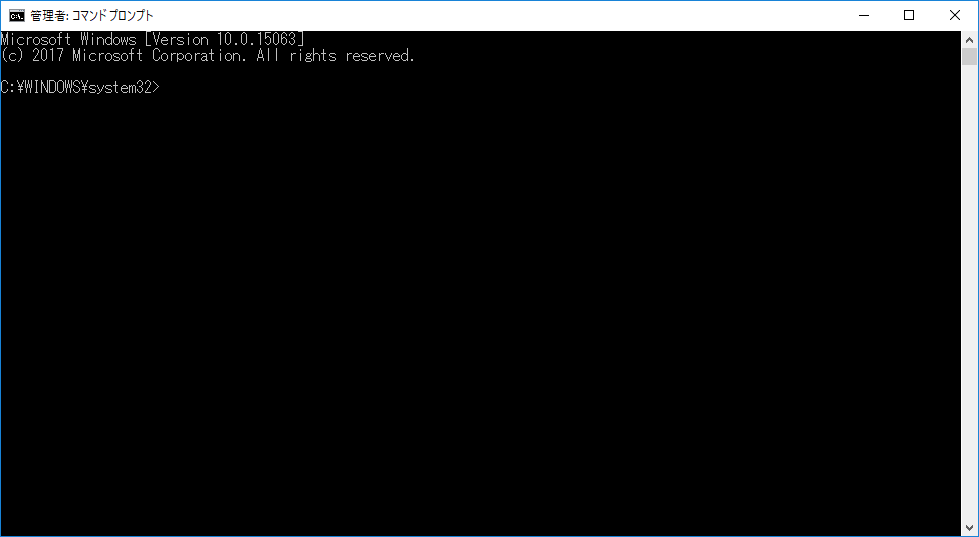
\includegraphics[width=12cm]{comand.PNG}
\caption{管理者で起動したコマンドプロンプト}\label{サンプル図}

\end{figure}


この画面から以下のコマンドを入力する.


\begin{verbatim}
@powershell -NoProfile -ExecutionPolicy Bypass -Command "iex ((New-Object
 System.Net.WebClient).DownloadString('https://chocolatey.org/install.ps1'))
" && SET "PATH=%PATH%;%ALLUSERSPROFILE%\chocolatey\bin"
\end{verbatim}

インストール終了後コマンドプロントを再起動して

\begin{verbatim}
clist
\end{verbatim}


と入力して,ソフトウェア一覧が表示されればインストール成功である.

\newpage





Chocolateyで使用できるコマンドは以下の通りである.なお,すべて省略されたコマンドである.


\begin{table}[htb]
   \caption{Chocolateyで使用できるコマンド}
  \begin{tabular}{|p{3cm}|p{9.5cm}|} \hline 
    cinst [パッケージ名] & 指定したパッケージをインストールする.インストールできるパッケージはChocolateyの公式サイトから確認できる. \\ \hline \hline
   cup [パッケージ名] & 指定したパッケージをアップデートする.allを指定すると全パッケージをアップデートする.逆に指定しなければChocolatey本体をアップデートする. \\ \hline
    cuninst [パッケージ名] & 指定したパッケージをアンインストールする.   \\ \hline
    clist & Chocoでインストールできるパッケージをすべて出力する. \\ \hline
    clist -lo [パッケージ名] & 指定したインストール済みのパッケージを出力する.パッケージ名を指定しなければすべてのパッケージを対象にする. \\ \hline
  \end{tabular}
\end{table}




\newpage

以下はホームページからインストールやパッケージの検索を行う方法.google検索でURL欄にhttps://chocolatey.org/ と入力してchocolateyのサイトを表示し,Install Chocolatey Nowをクリックする.


\begin{figure}[h]
\centering
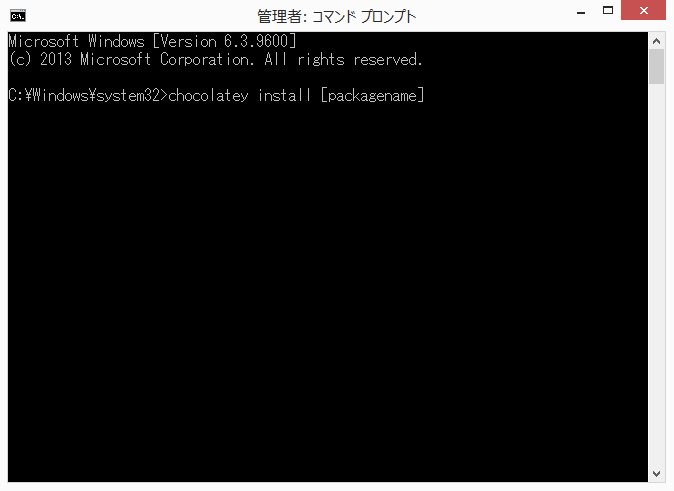
\includegraphics[width=12cm]{choco.PNG}
\caption{Chocolateyダウンロードサイト}\label{サンプル図}
\end{figure}


その後画像のmore optionsを選択.その後,インストールに使うアプリケーションに応じたコマンドをコピーする.パッケージページに飛ぶと,Chocoでインストールできるパッケージを検索し,インストールのコマンドを知ることもできる.

\begin{figure}[h]
\centering
\includegraphics[width=12cm]{chocoMoreoption.PNG}
\caption{Chocolateyダウンロードサイト}\label{サンプル図}
\end{figure}




\newpage

\begin{figure}[h]
\centering
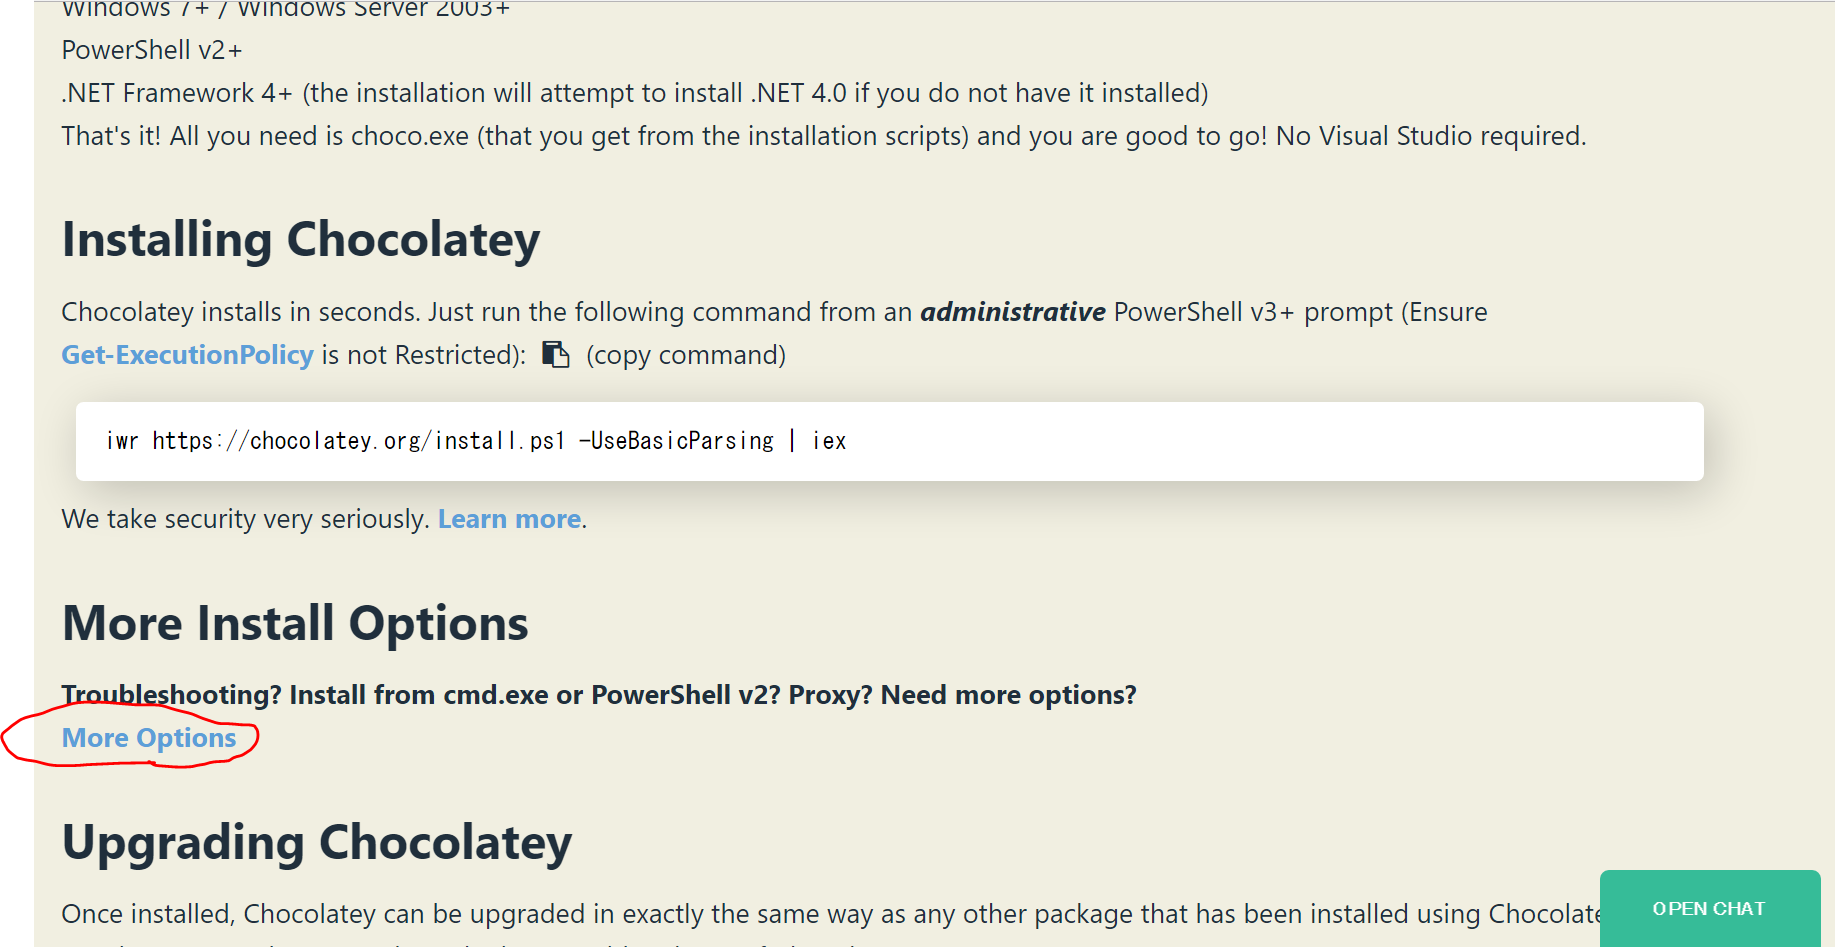
\includegraphics[width=12cm]{choco2.PNG}
\caption{Chocolateyにあるコマンドコード}\label{サンプル図}
\end{figure}
Install with cmd.exeに書かれているコマンドをコピーする.

\begin{figure}[h]
\centering
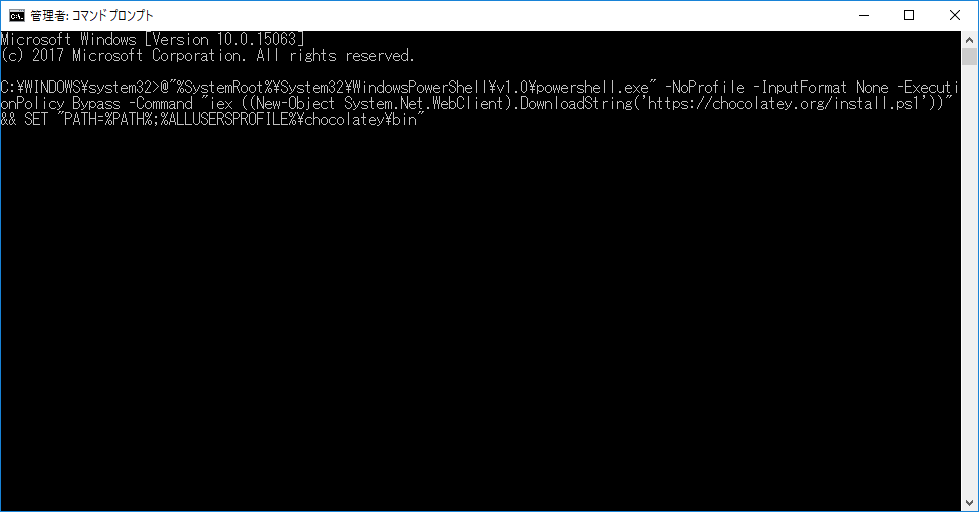
\includegraphics[width=12cm]{comand2.PNG}
\caption{管理者権限のコマンドプロント}\label{サンプル図}
起動した管理者権限のコマンドプロントにコピーしたコードをペーストして実行する.
\end{figure}
\newpage



\section{VirtualBoxについて}
\subsection{VirtualBoxとは}
VirtualBoxは,使用しているPC上に仮想のPCを作成し,別のOSをインストール・実行できるフリーの仮想化ソフトである.

VirtualBoxはコンピューター上で直接動作している通常のOSにとってはアプリケーションソフトの一つであり,他のソフトと同じように起動することができる.起動すると仮想的なコンピューターが構築され,元のOSとは独立に別のOSを起動することができる.VirtualBoxが実行されているOSをホストOS,VirtualBox上で実行されているOSをゲストOSという.

\begin{figure}[h]
\centering
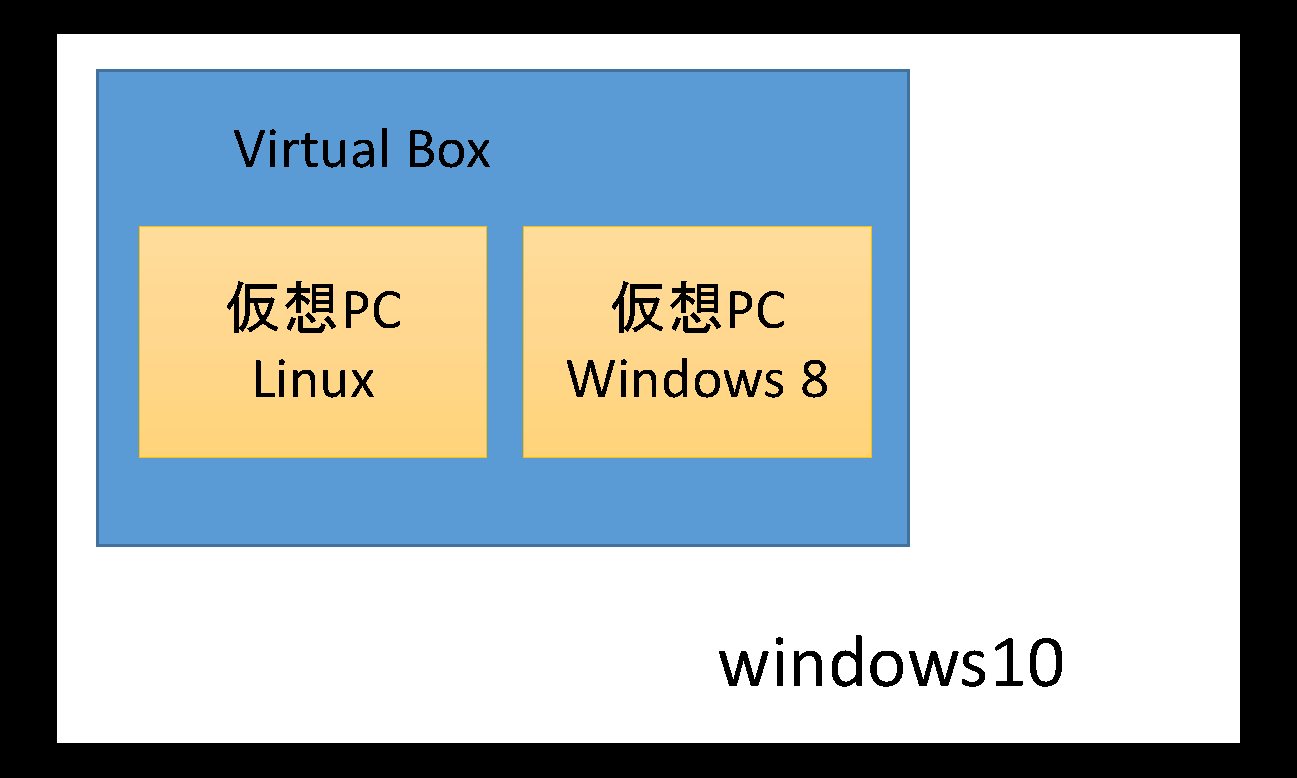
\includegraphics[width=12cm]{virtualbox.pdf}
\caption{仮想マシンのイメージ}\label{サンプル図}
\end{figure}

元は独立系のソフトウェア企業が開発・販売していた製品だったが,開発元がSumMicrosy stems社に買収されたため,Oracle社が開発元となり,正式名称も「Oracle NM VirtualBox」となった.また,VirtualBox本体はGPLに基づいてオープンソースソフトウェアとして公開され,誰でも自由に入手・利用・改変・再配布などが行える.同社ではVirtualBoxに機能を追加するソフトウェアを製品として開発・販売している.
\newpage


\subsection{VirtualBoxのインストール}
ChocolateyのサイトでVirtualBoxと入力して検索する.

\begin{figure}[h]
\centering
\includegraphics[width=12cm]{chocoSearch.PNG}
\caption{VirtualBoxのインストール}\label{サンプル図}
\end{figure}



\newpage



検索結果の上位にVirtualBoxのパッケージが出てくるので,右側にある黒い部分のvirtualboxをインストールするためのコマンドをコピーする.

\begin{figure}[h]
\centering
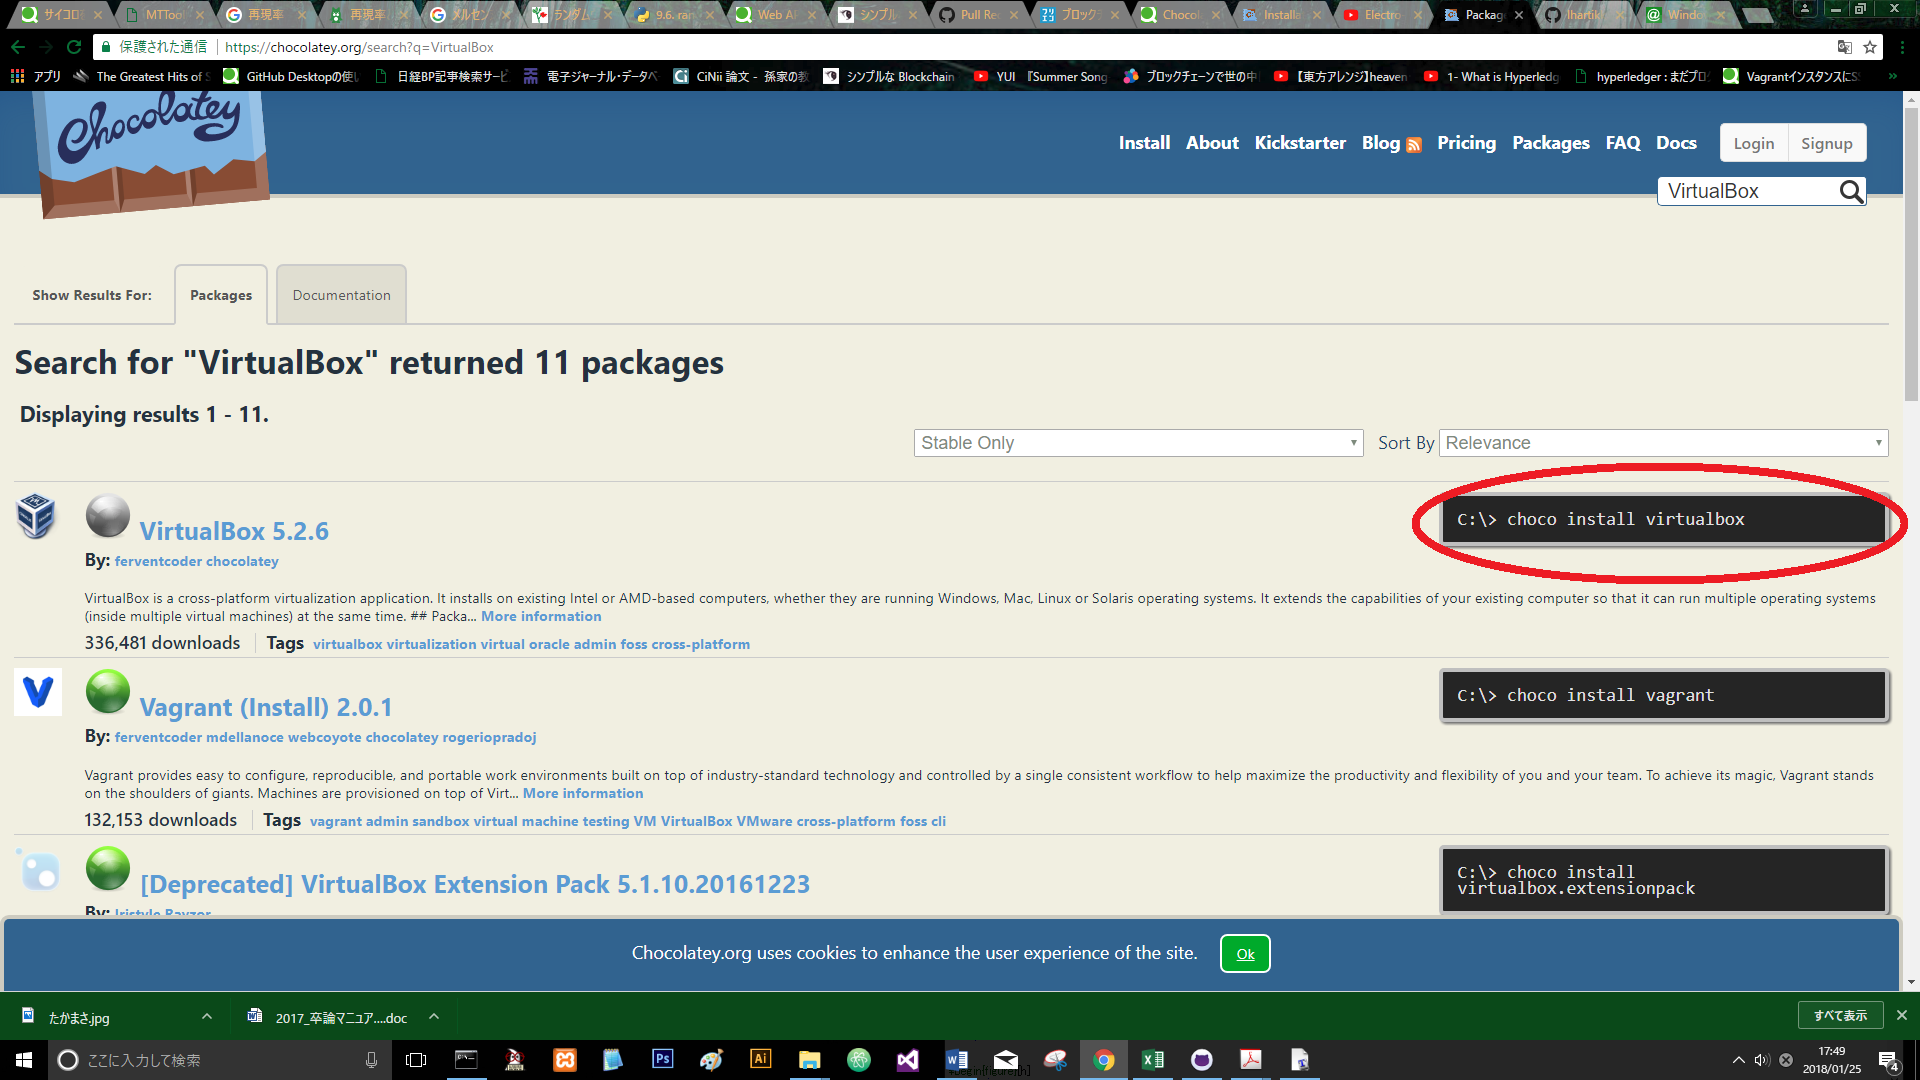
\includegraphics[width=12cm]{chocoVirt.PNG}
\caption{VirtualBoxのインストール}\label{サンプル図}
\end{figure}




\newpage


コマンドプロントを管理者で起動して,コピーしたchoco install virtualboxというコマンドをペーストして実行するとインストールが開始される.

\begin{figure}[h]
\centering
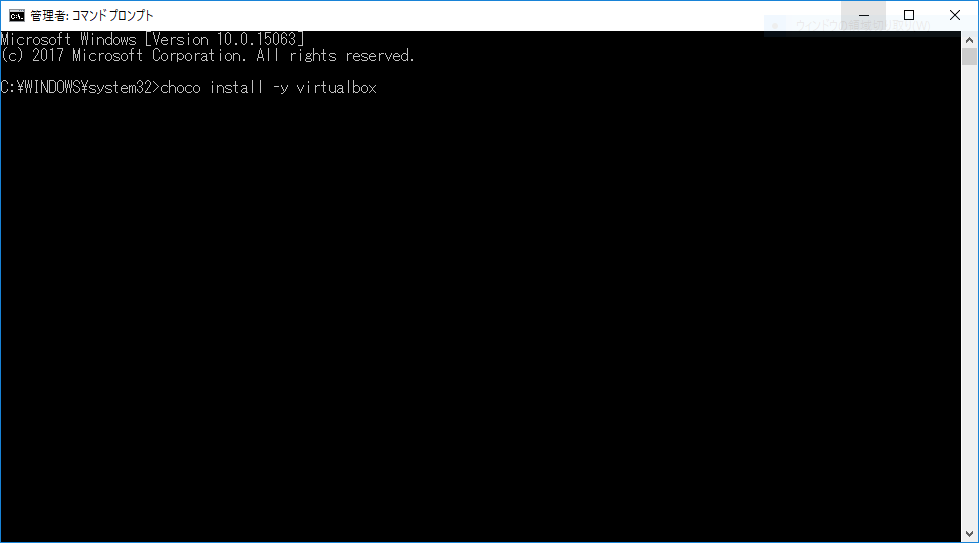
\includegraphics[width=12cm]{virtualboxinstall.PNG}
\caption{VirtualBoxのインストール}\label{サンプル図}
\end{figure}
\newpage


またchoco install -y virtualbox と入力し実行すると一度にインストールが終わる.
\begin{figure}[h]
\centering
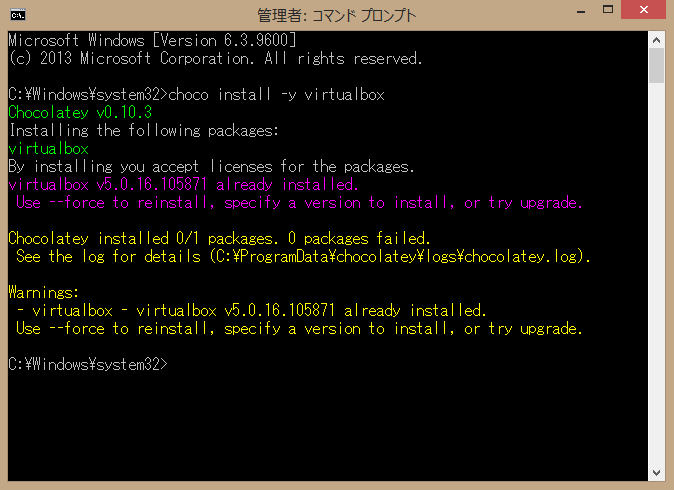
\includegraphics[width=12cm]{virtualboxinstall2.PNG}
\caption{VirtualBoxのインストール}\label{サンプル図}
\end{figure}

このようになればインストール完了.
\newpage


\section{Vagrantについて}
\subsection{Vagrantとは}
Vagrantとは,仮想環境を作成するにあたって,簡単に構築・管理し配布することができるツールである.

Vagrantを使うには,Boxと呼ばれるファイルが必要になる.今回は,矢吹研究室の公式マシンを使用する.

矢吹研究室公式マシンは以下のURLのGithubリポジトリで公開されており,このリポジトリをcloneして使用する.なお,矢吹研究室公式マシンはLinuxディストリビューションの一つであるUbuntuを使用している.

https://github.com/yabukilab/machine


\newpage


\subsection{Vagrantのインストール}
ChocolateyのサイトでVagrantと入力して検索する.

\begin{figure}[h]
\centering
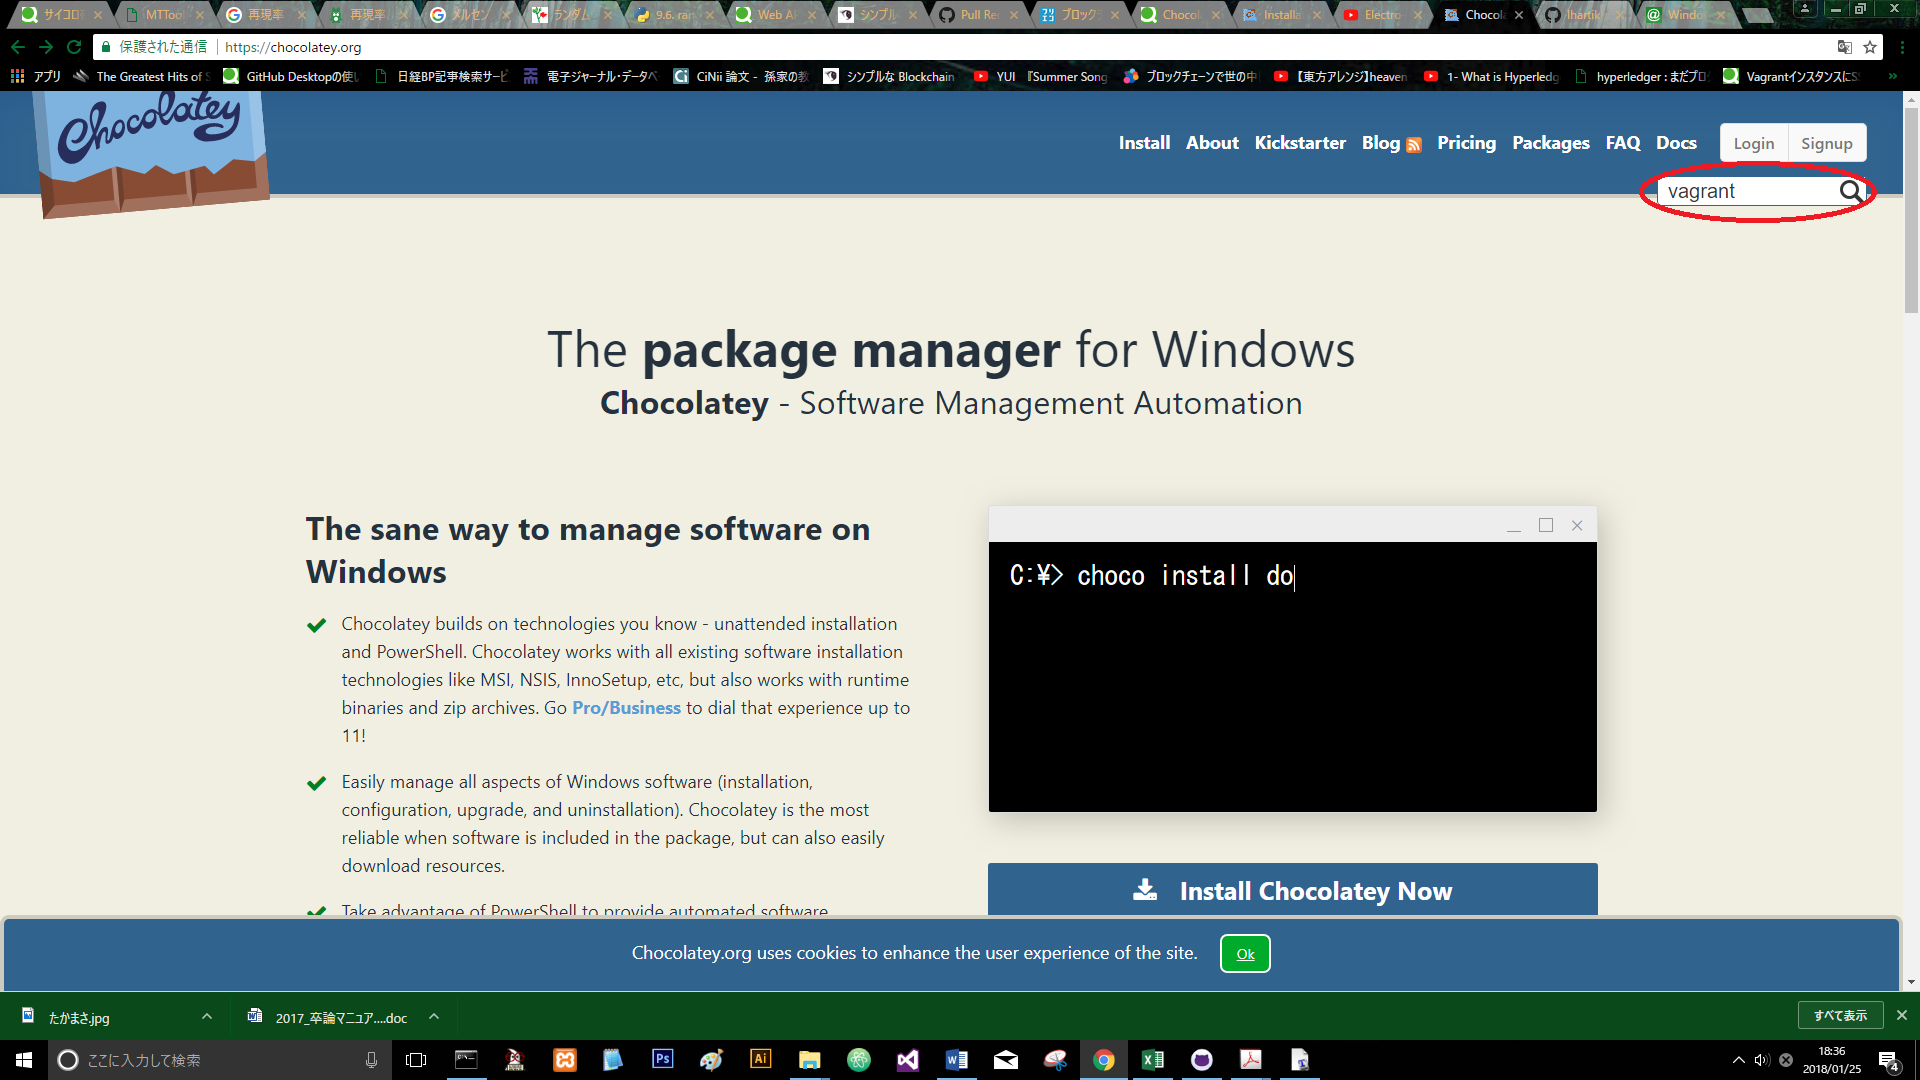
\includegraphics[width=12cm]{vagrantsearch.PNG}
\caption{Vagrantのインストール}\label{サンプル図}
\end{figure}


\newpage

検索の上位にVagrantのパッケージが出てくるので,右側にある黒い部分のVagrantをインストールするためのコマンドをコピーする.
\begin{figure}[h]
\centering
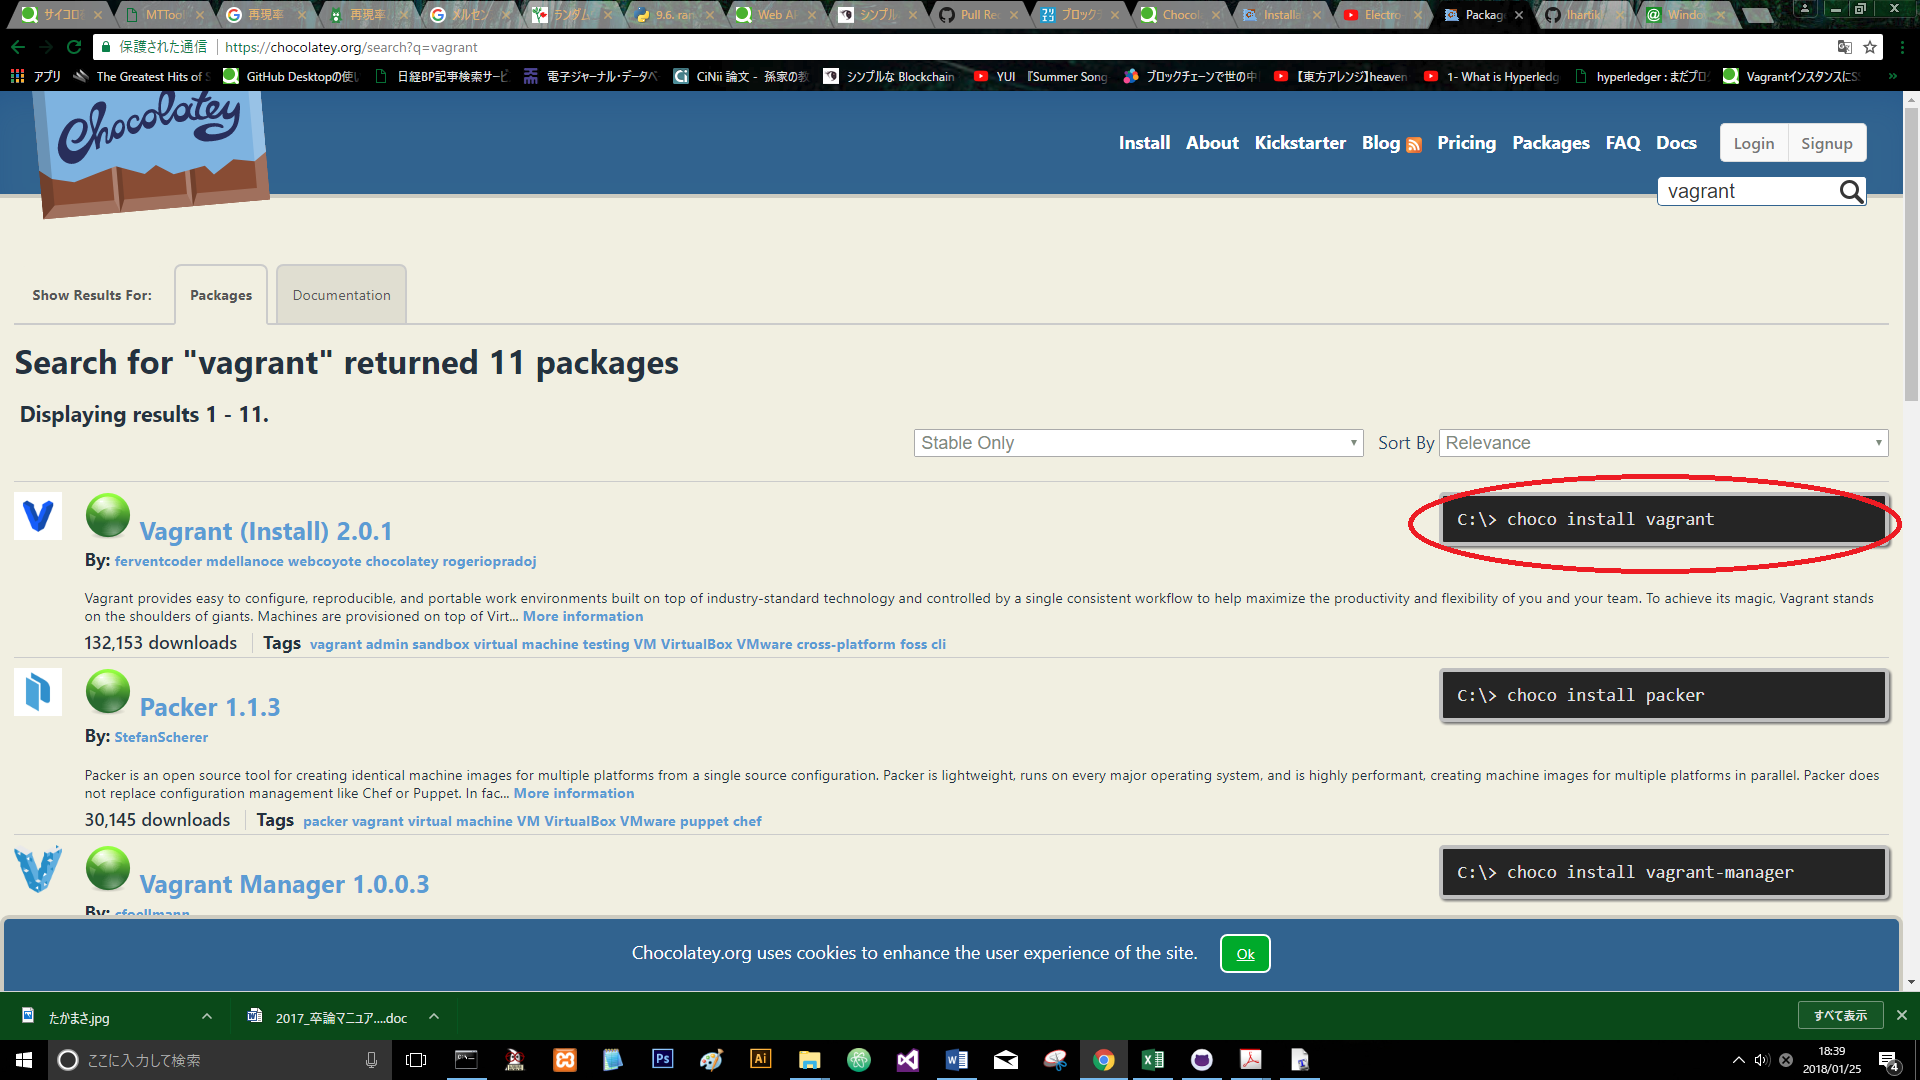
\includegraphics[width=12cm]{vagrantkopi.PNG}
\caption{Vagrantのインストール}\label{サンプル図}
\end{figure}


\newpage

コマンドプロントを管理者で起動して,コピーした choco install vagrant というコマンドをペーストして実行するとインストールが開始される.

\begin{figure}[h]
\centering
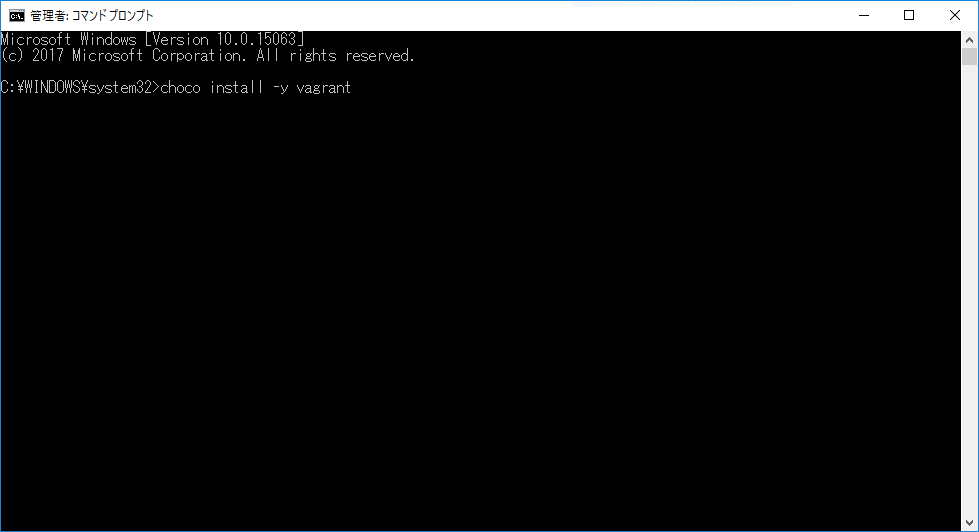
\includegraphics[width=12cm]{vagrant.PNG}
\caption{Vagrantのインストール}\label{サンプル図}
\end{figure}


\newpage

また,choco install -y vagtrantと入力し実行すると一度にインストールが終わる.
\begin{figure}[h]
\centering
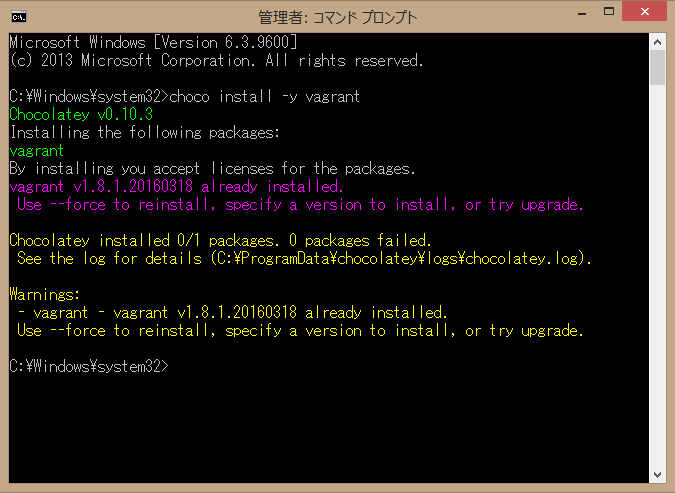
\includegraphics[width=12cm]{vagrant2.PNG}
\caption{Vagrantのインストール}\label{サンプル図}
\end{figure}

このようになればインストール成功.

\newpage


\subsection{データ通信解除}

Vagrantfileをテキストエディタで開いて37行目にあるコメントアウトを削除する.この行為によって同一ネットワーク上でのデータ通信が解除される.
Vagrantfileの場所は以下の通りである.

\begin{verbatim}
c/vagrant/machine/Vagrantfile
\end{verbatim}

\begin{figure}[h]
\centering
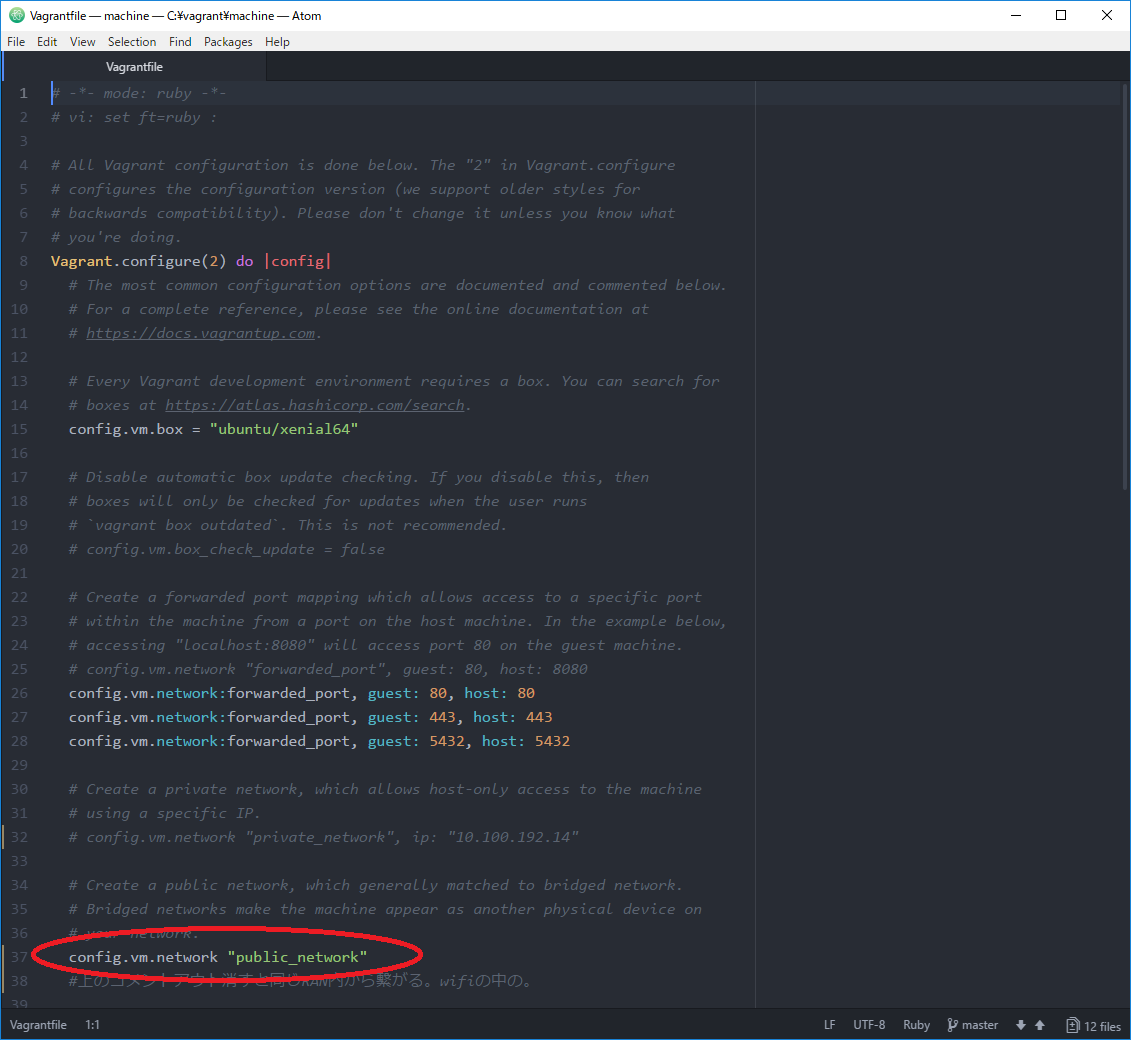
\includegraphics[width=12cm]{komenntoout.PNG}
\caption{コメントアウトの削除}\label{サンプル図}
\end{figure}

\newpage




\subsection{計算機環境の構築}
VagrantのBoxを用意する.今回は矢吹研究室の公式仮想マシンを用いる.管理者権限のないコマンドプロンプトを起動し,以下のコマンドを入力する.

仮想マシンの再構築を高速にするために,キャッシュを導入する.

\begin{verbatim}
vagrant plugin install vagrant-cachier
\end{verbatim}

仮想マシンを用意する
\begin{verbatim}
cd \
mkdir vagrant
cd vagrant
git clone https://github.com/yabukilab/machine.git
\end{verbatim}
\newpage

起動
\begin{verbatim}
cd vagrant
cd machine
vagrant up
\end{verbatim}

Vagrantが起動に成功したか確認する方法.ブラウザのURL入力欄に以下のURLを入力してアクセスできるか確認する.
\begin{verbatim}
http://localhost/phpmyadmin/
ユーザ名 root
パスワード pass
\end{verbatim}


\begin{figure}[h]
\centering
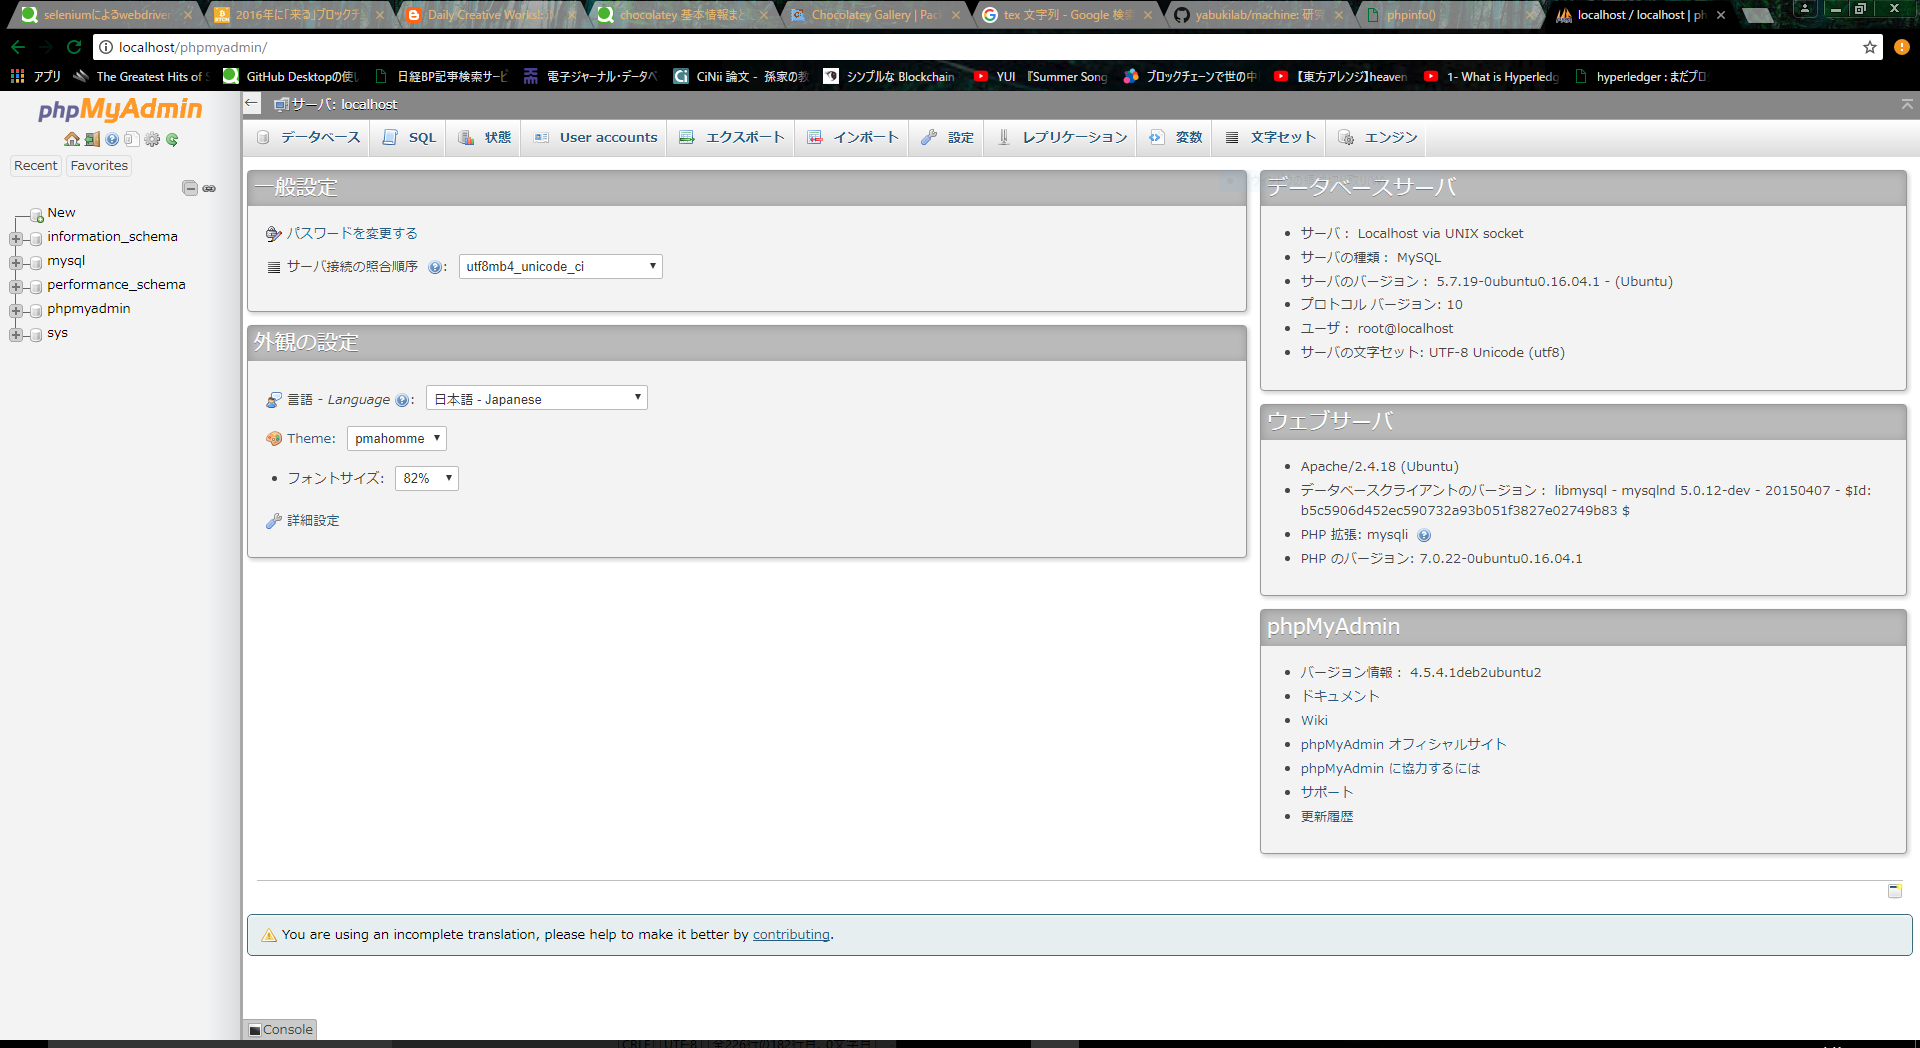
\includegraphics[width=12cm]{php.PNG}
\caption{vagrant起動成功確認画面}\label{サンプル図}
\end{figure}


仮想マシンの再起動と停止,削除.
\begin{verbatim}
・再起動:  vagrant reload
・停止:     vagrant halt
・削除:     vagrant destroy
\end{verbatim}

\newpage

接続
\begin{verbatim}
vagrant ssh
\end{verbatim}

\begin{figure}[h]
\centering
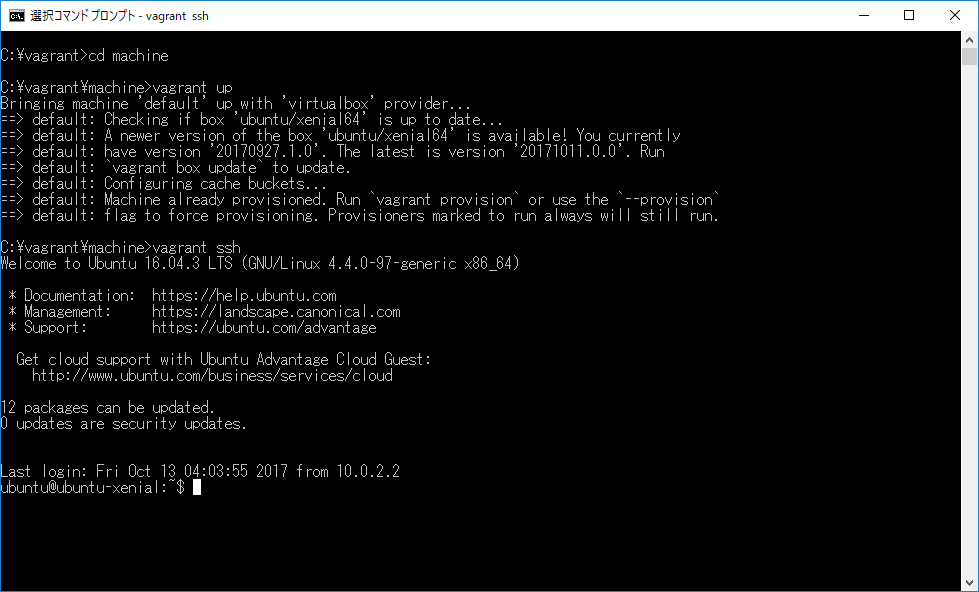
\includegraphics[width=12cm]{vagrantssh.PNG}
\caption{Vagrantssh接続}\label{サンプル図}
\end{figure}

このように表示されれば接続成功.

また,やり直したい場合は以下のコマンドを実行する.
\begin{verbatim}
c \
cd vagrant
cd machine
cd destroy
cd ..
rmdir /S /Q machine
\end{verbatim}

\newpage



\section{dockerについて}
\subsection{dockerとは}
dockerとはコンテナ型の仮想化環境を提供するオープンソフトウェアである.VMware製品などの完全仮想化を行うハイパーバイザ型製品と比べて,ディスク使用量が少なく,仮想環境(インスタンス)作成や起動は速く,性能劣化がほとんどないという利点を持つ.naivechainを動かすにはまずdockerをインストールしなければならない.

\subsection{リソースの効率化}
一台のサーバ上に複数のオペレーティングシステム(OS)を走らせる仮想化技術は従来から存在していた.例えばハイパーバイザ型のHyper-Vやホスト型のVirtualBox等である.仮想化の本来の目的は,一台のハードウエア内に出来る限り多くのアプリケーションを実行する事であるが,上記種類の仮想化では仮想環境毎にOSを丸ごとインストールする必要があり,アプリケーションに必要のないサービスやファイルまで伴っていた.これはリソースの無駄使いであった.

アプリケーションとは直接関係の無いライブラリやデータは仮想環境内で共有する事が望ましかった.これを実現するのがコンテナ型の仮想化である。実際にDockerは、ホストOSのカーネルを共有する。それぞれの仮想環境はDockerコンテナと呼ばれ,一台のサーバ上でそれぞれが隔離される事で複数のインスタンスが動作しているように見える.


\subsection{アプリ実行環境の容易さ}
一般にアプリケーションを開発もしくは動作させるまでには,設定ファイルの編集や必要なライブラリのインストール等,本来の目的には関係のない煩雑な作業が必要である.Dockerはアプリケーションとライブラリを同一のコンテナ内に固めてしまう.一度固めたコンテナは軽量であるため移動が容易であり,比較的どの環境でも素早く目的のアプリケーションを動作させる事が可能である.これをDocker社は,Build,Ship,and Run Any App,Anywhere と表現している\cite{d}.

\subsection{dockerの評価}
Dockerのコンテナー管理の手軽さやインスタンス操作の高速性は,クラウドサービスやビッグデータ基盤などを管理するためのIT基盤として高く評価され,2014年12月日経BP社より「ITインフラテクノロジーAWARD 2015」グランプリに選出されている.


日本では「Immutable Infrastructure(不変のインフラ)」という表現と共に話題になることが多い.


2014年,GoogleはDockerとは言及していないが,コンテナ型仮想技術を利用しており,毎週20億個のコンテナを自社サービスのために起動していると発表した.


\newpage

\subsection{dockerのインストール}
上記のvagrant sshを行って仮想マシンに接続した状態でdockerのインストールを行う.以下のコマンドを実行する.

\begin{verbatim}
sudo apt-get install docker.io -y
\end{verbatim}

\begin{figure}[h]
\centering
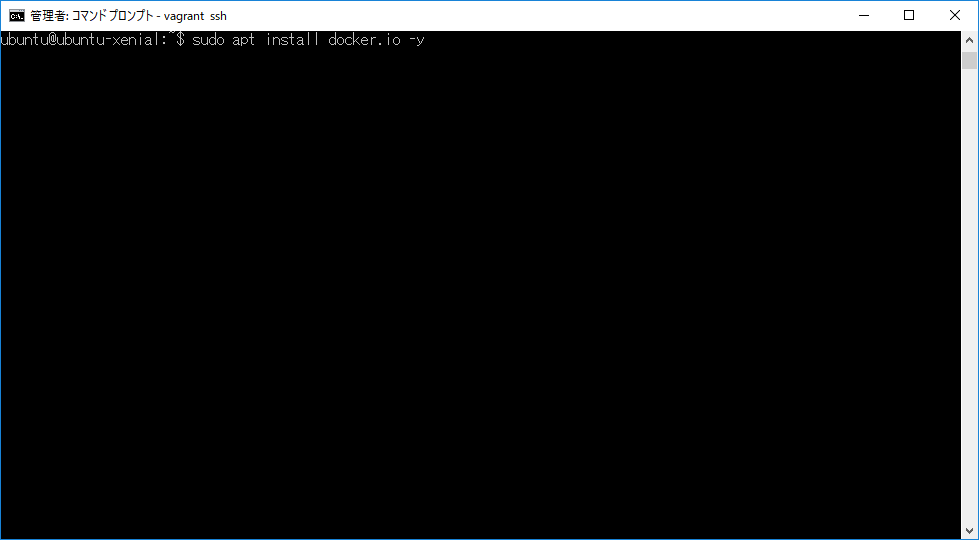
\includegraphics[width=12cm]{dockerinstall.png}
\caption{dockerのインストール}\label{サンプル図}
\end{figure}


\begin{figure}[h]
\centering
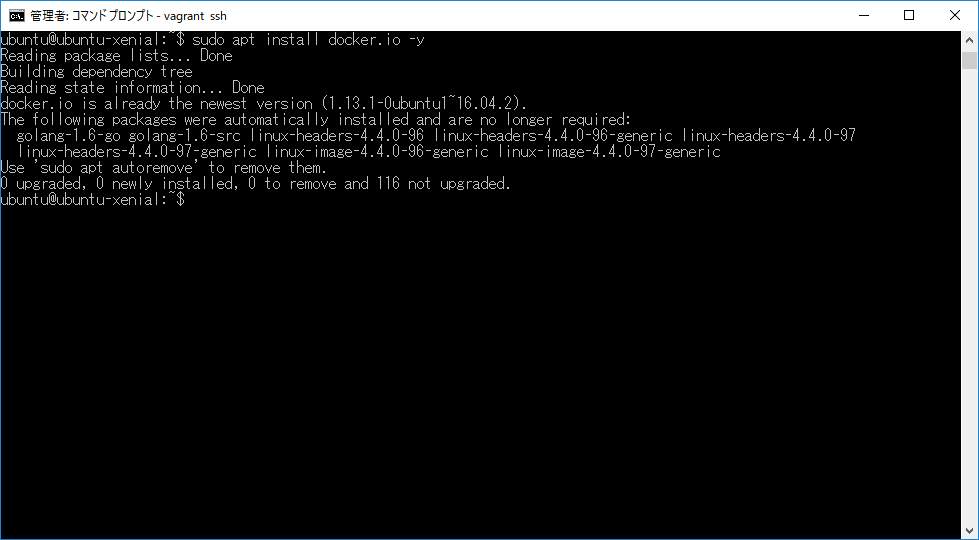
\includegraphics[width=12cm]{dockerinstall2.png}
\caption{dockerのインストール}\label{サンプル図}
\end{figure}


このように表示されればインストール成功.

\newpage


dockerのバージョンを確認する場合は以下のコマンドを実行する.

\begin{verbatim}
docker version
\end{verbatim}


\begin{figure}[h]
\centering
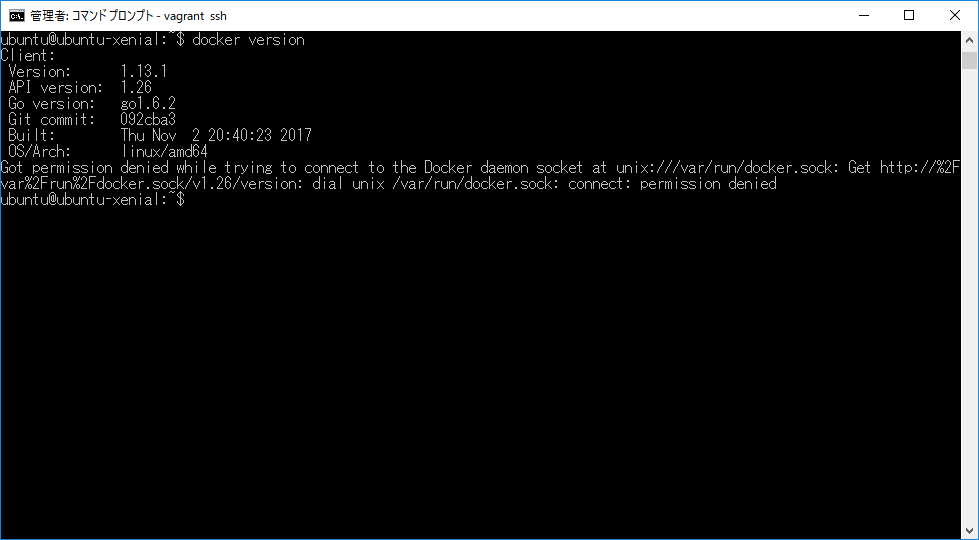
\includegraphics[width=12cm]{dockerversion.png}
\caption{dockerのバージョン確認}\label{サンプル図}
\end{figure}


このように表示されればdockerのversionがわかる.

\newpage


\section{docker composeについて}

\subsection{docker composeとは}
docker composeとはdockerコンテナの管理を支援する純正ツールである.Docker ComposeはDockerが開発するコマンドラインツールで,あらかじめ用意しておいた設定ファイルに従ってコンテナを起動するツールだ.設定ファイルには複数のコンテナに関する記述が可能で,コンテナの起動オプションやコンテナに与える環境変数など,さまざまな設定も同時に記述できる\cite{e}.


また,コンテナ同士の依存関係を設定することも可能で,これによって関連するコンテナを複数まとめて起動することも可能だ.


ここでこの画像を入れる



\subsection{docker composeの利用ケース}
Docker Composeを活用できるケースとしては,まずソフトウェアの開発/テスト環境が挙げられる.昨今ではデータベースやキャッシュ,フロントエンドといった役割毎に複数のサーバーを用意し,それらを組み合わせてサービスを構築する例が多い.こういった場合,開発/テスト環境でもそれらをすべて用意する必要がある.それらをコンテナの形で用意しておき,それらを起動するためのオプション設定などをDocker Composeの設定ファイルに記述しておけば,コマンドを1つ実行するだけでテスト環境を立ち上げられるようになる.


また,7月末にリリースされたDocker 1.12では「docker stack」という機能が実験的に導入された.これを利用することで,Docker Compose向けに定義したコンテナの設定等をそのまま利用してDockerクラスタ内でコンテナを稼動させられるようになる.これにより,Docker Composeを使って作ったテスト環境を,容易に実運用環境に移行させられるようになることが期待される.




\newpage



\subsection{Docker Composeのインストール方法}

dockerのインストールが終わっている仮想マシンで以下のコマンドを実行する.


\begin{verbatim}
sudo apt-get install docker-compose -y
\end{verbatim}


\begin{figure}[h]
\centering
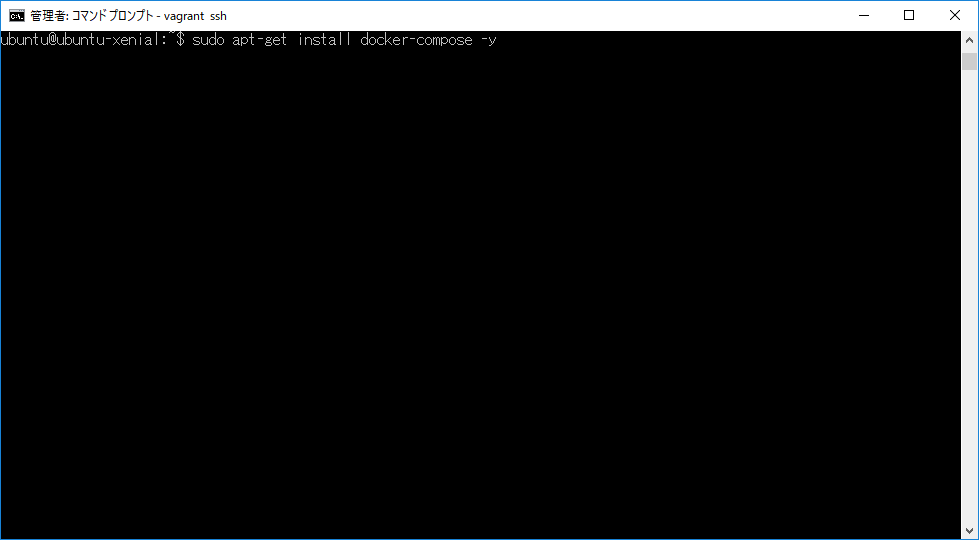
\includegraphics[width=12cm]{dockercomposeinstall.PNG}
\caption{docker composeのインストール}\label{サンプル図}
\end{figure}

\begin{figure}[h]
\centering
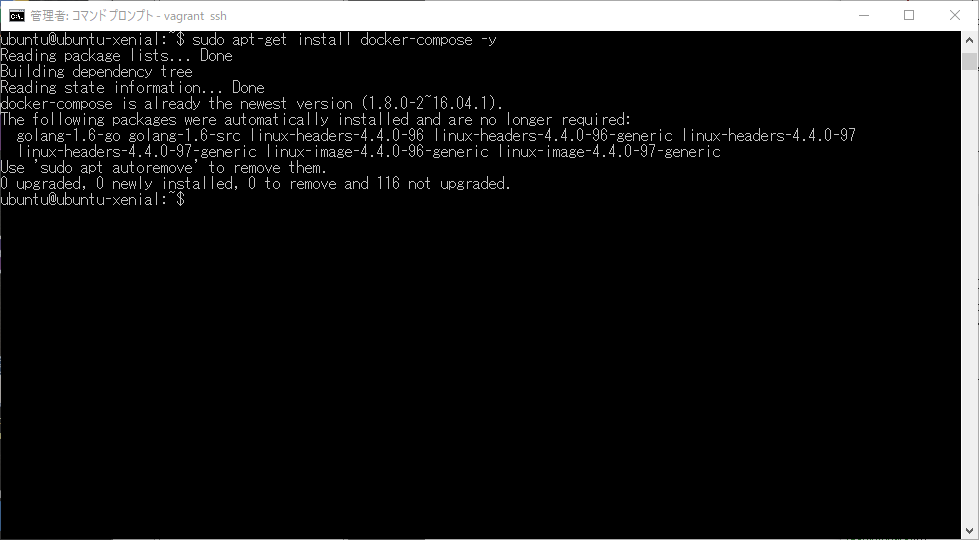
\includegraphics[width=12cm]{dockercomposeinstall2.PNG}
\caption{docker composeのインストール}\label{サンプル図}
\end{figure}

このように表示されればdocker composeのインストール成功.


\newpage



docker composeのバージョンを確認する場合は以下のコマンドを実行する.

\begin{verbatim}
docker-compose -v
\end{verbatim}



\begin{figure}[h]
\centering
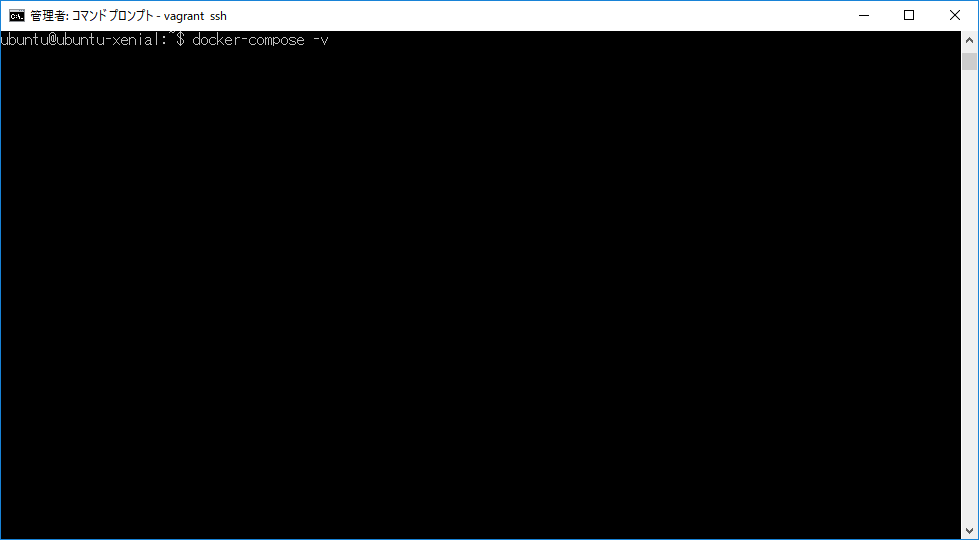
\includegraphics[width=12cm]{dockercomposeversion.PNG}
\caption{docker composeのバージョン確認}\label{サンプル図}
\end{figure}



\begin{figure}[h]
\centering
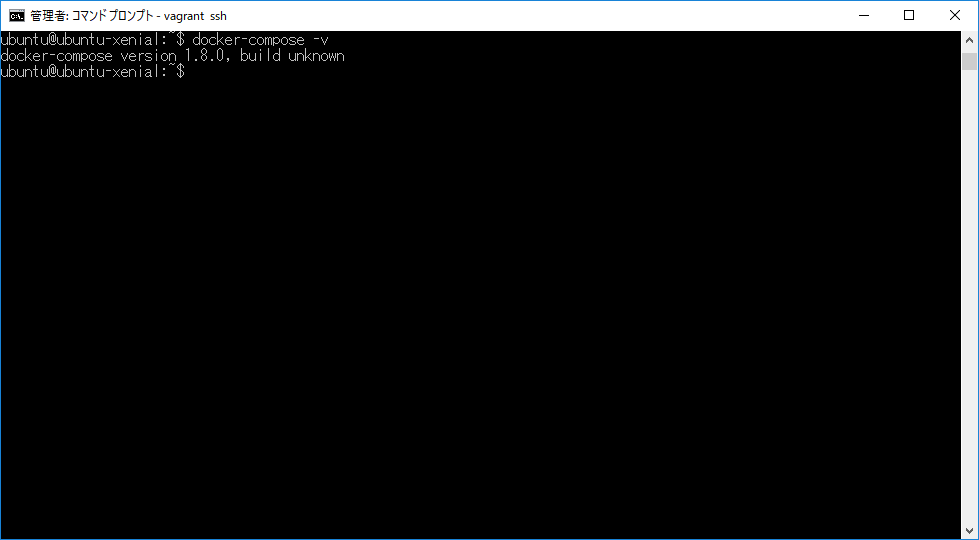
\includegraphics[width=12cm]{dockercomposeversion2.PNG}
\caption{docker composeのバージョン確認}\label{サンプル図}
\end{figure}


このように表示されればdocker-composeのversionがわかる.



\newpage


\section{naivechainについて}

\subsection{naivechainとは}
ブロックと呼ばれるデータが順序つけられた200行のjavascriptに実装した非常にシンプルなブロックチェーンである.
naivechainではインデックス,タイムスタンプ,データ,ハッシュ値,そして一つ前のブロックのハッシュ値のみの構造である.
\begin{figure}[h]
\centering
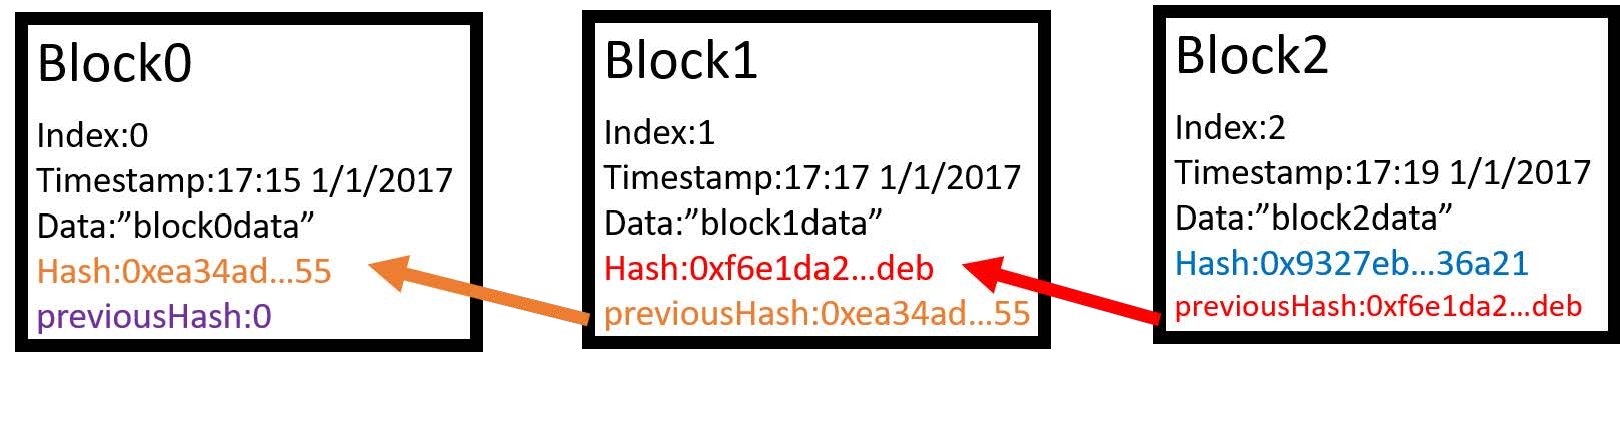
\includegraphics[width=12cm]{naivechain.pdf}
\caption{naivechainのイメージ}\label{サンプル図}
\end{figure}

\newpage





\subsection{パッケージリストの更新}
まず,先に述べた仮想マシンに接続した状態から以下のコマンドでパッケージリストの更新を行う.
sudo apt-get update

\begin{figure}[h]
\centering
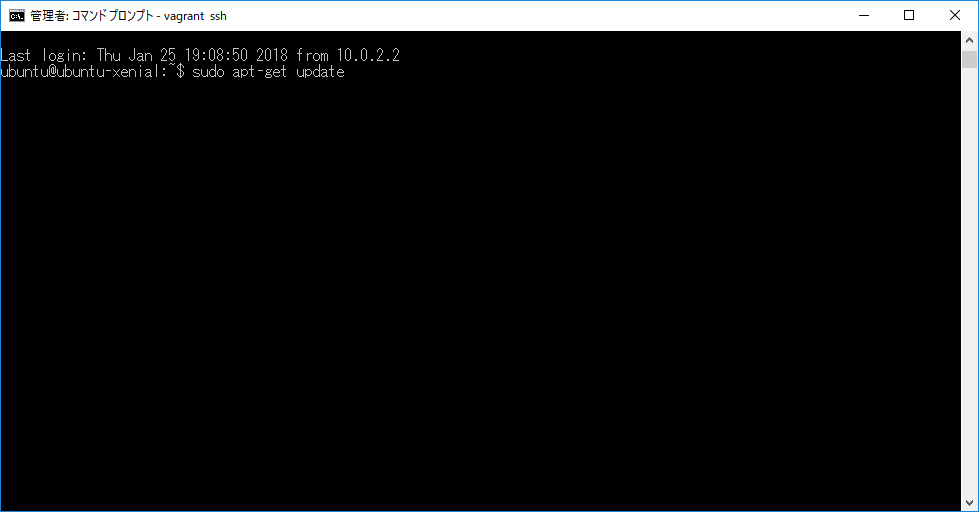
\includegraphics[width=12cm]{sudoaptupdate.PNG}
\caption{パッケージリストの更新}\label{サンプル図}
\end{figure}

パッケージリストのアップデート完了画面.
\begin{figure}[h]
\centering
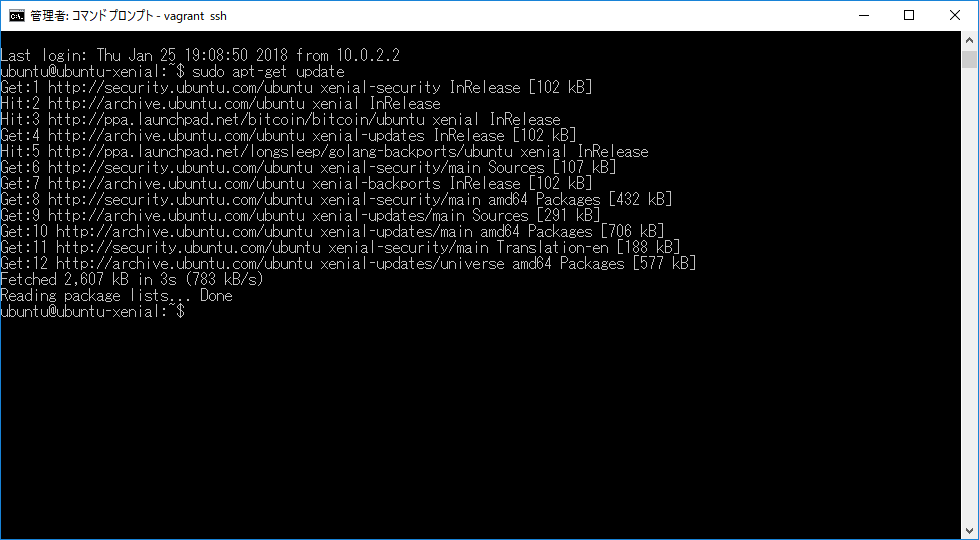
\includegraphics[width=12cm]{sudoupdate.PNG}
\caption{パッケージリストの更新}\label{サンプル図}
\end{figure}


\newpage

\subsection{naivechainのインストール}

docker,docker composeのインストールが終わっている仮想マシンで以下のコマンドを実行する.

\begin{verbatim}
git clone https://github.com/lhartikk/naivechain
\end{verbatim}


naivechainのファイルへ移動するために以下のコマンドを実行する.

\begin{verbatim}
cd naivechain
\end{verbatim}

\begin{figure}[h]
\centering
\includegraphics[width=12cm]{cdnaivechain.PNG}
\caption{パッケージリストの更新}\label{サンプル図}
\end{figure}


\newpage


\begin{figure}[h]
\centering
\includegraphics[width=12cm]{cdnaivechain2.PNG}
\caption{パッケージリストの更新}\label{サンプル図}
\end{figure}


このように表示されればnaivechainファイルへの移動成功である.


\newpage


\subsection{naivechainの起動}


naivechainを実行するために以下のコマンドを実行する.
\begin{verbatim}
sudo docker-compose up
\end{verbatim}



\begin{figure}[h]
\centering
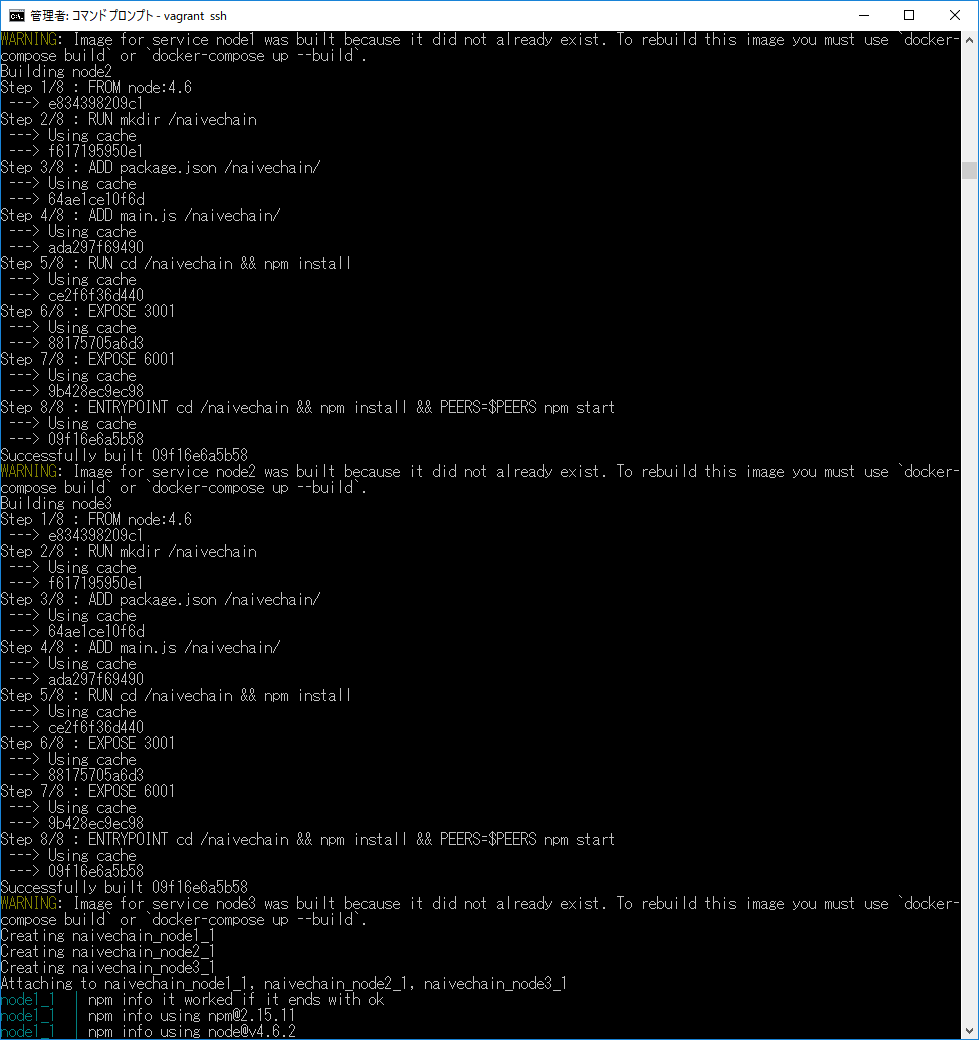
\includegraphics[width=12cm]{composeup.PNG}
\caption{compose up 成功画面}\label{サンプル図}
\end{figure}

\newpage

\begin{figure}[h]
\centering
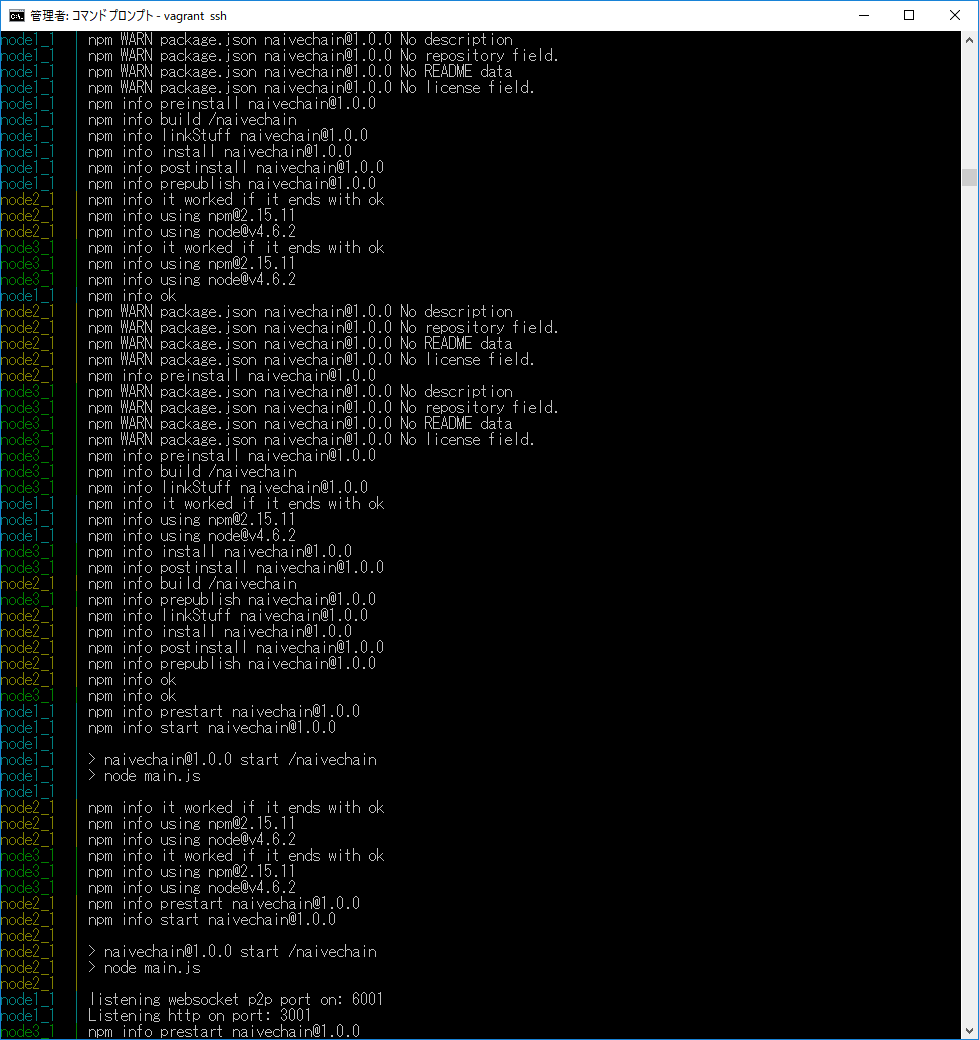
\includegraphics[width=12cm]{composeup2.PNG}
\caption{compose up 成功画面}\label{サンプル図}
\end{figure}


\newpage


\begin{figure}[h]
\centering
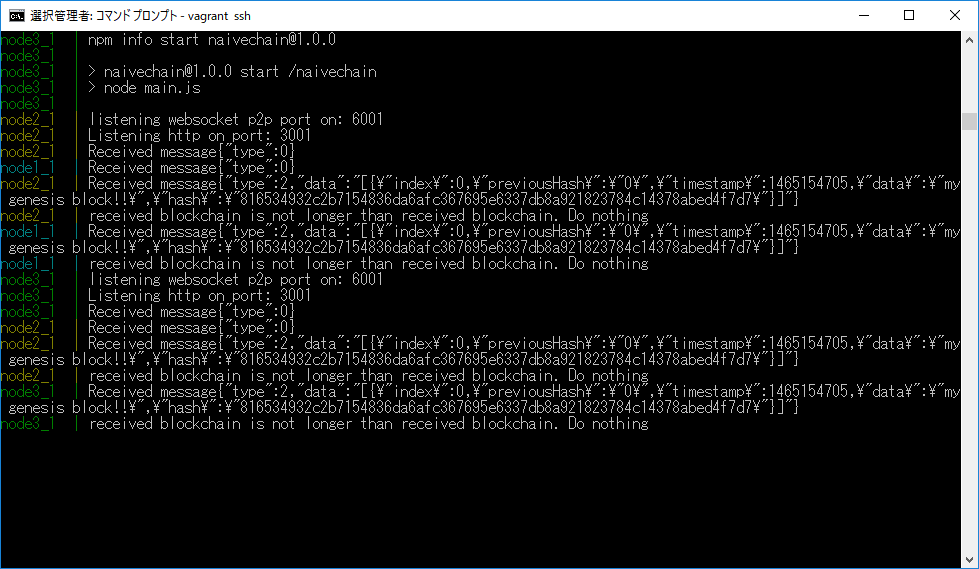
\includegraphics[width=12cm]{composeup3.PNG}
\caption{compose up 成功画面}\label{サンプル図}
\end{figure}


このように表示されればdocker compose の起動成功である.naivechainを使用することができる.


\newpage


\subsection{ipアドレス確認}

naivechainを用いる際に,自分のノードがホストノードとなって他ノードから自分のノードへブロックを追加する場合,自分のipアドレスを確認する必要がある.そのため以下のコマンドを実行してipアドレスを確認する必要がある.


\begin{verbatim}
ifconfig
\end{verbatim}

\begin{figure}[h]
\centering
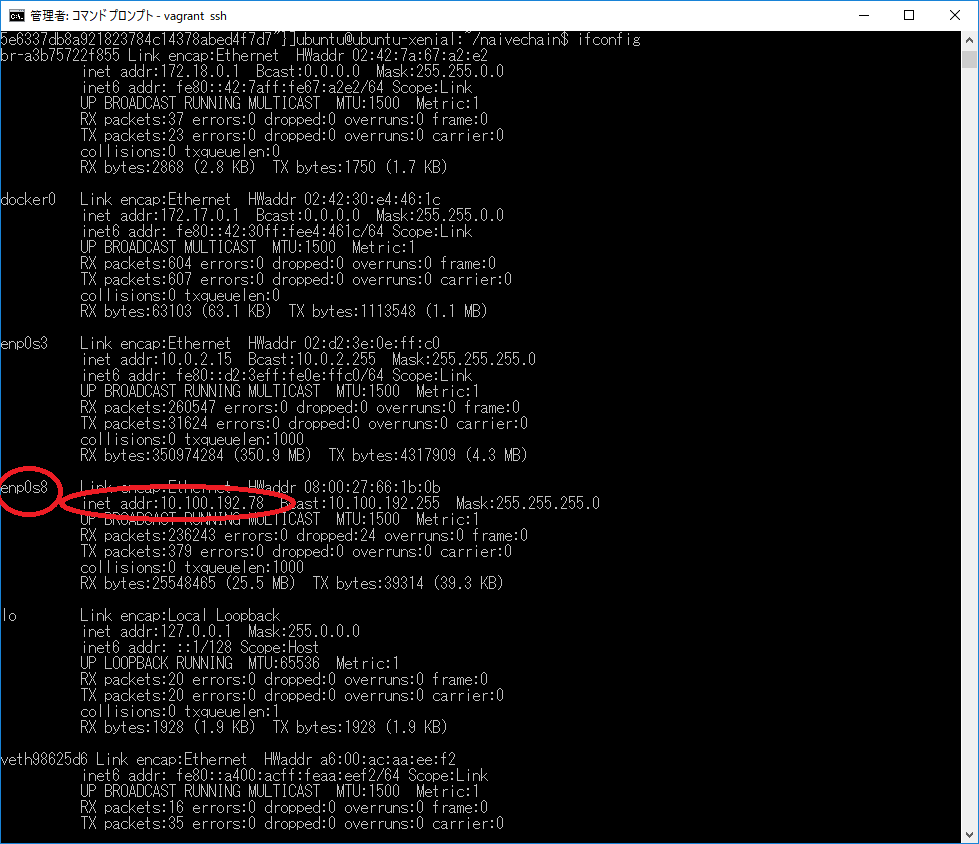
\includegraphics[width=12cm]{ifconfig.PNG}
\caption{ipアドレス確認}\label{サンプル図}
\end{figure}



\begin{verbatim}
enp0s8
inet addr:10.100.192.78
\end{verbatim}

赤い丸で囲った部分が自分のipアドレスである.

\newpage




\section{Bitcoin Coreについて}

Bitcoin CoreはBitcoinクライアントのリファレンス実装であり,公式リポジトリから誰でもダウンロードして利用することができる.ビットコインのBTCは取引所を介してインターネット上で売買されているため,本プログラムを使用すれば,本物のビットコインの送金や,マイニングが可能になる\cite{b}.


ここではOracle社製の仮想ソフトウェアであるVirtualBoxを使用してWindowsをホストOSとした環境上にゲストOSとしてUbuntuを導入し,その上にブロックチェーン環境を構築する.


\subsection{Bitcoin Coreののソースコード・ライブラリの取得}

\begin{verbatim}
mkdir src
cd src
git clone https://github.com/bitcoin/bitcoin.git
\end{verbatim}


\subsection{パッケージリストの更新}

\begin{verbatim}
sudo apt-get update
\end{verbatim}


\newpage


\subsection{gccをインストール}

\begin{verbatim}
sudo apt-get install build-essential libtool autotools-dev automake pkg-config 
 libssl-dev libevent-dev bsdmainutils
\end{verbatim}


\subsection{OpenSSLをインストール}
\begin{verbatim}
sudo apt-get install libtool autotools-dev autoconf
sudo apt-get install libssl-dev
\end{verbatim}


\subsection{gccをインストール}
\begin{verbatim}
sudo apt-get install libboost-all-dev
\end{verbatim}


\subsection{libd4.8をインストール}
\begin{verbatim}
sudo apt-get-repository ppa:bitcoin/bitcoin
sudo apt-get update
sudo apt-get install libd4.8-dev
sudo apt-getinstall libqrencode-dev
\end{verbatim}


\subsection{関連ライブラリをインストール}
\begin{verbatim}
sudo apt-get install libminiupnpc-dev
sudo apt-get install libqrencode-dev
\end{verbatim}


\subsection{GUIライブラリをインストール}
\begin{verbatim}
sudo apt-ghet install libqt5gui5 libqt5core5a libqt5dbus5
 qttools5-dev qttools-dev-tools
libprotobuf-dev protobuf-compiler
\end{verbatim}


\newpage


\subsection{Bitcoin Coreのビルド}
\begin{verbatim}
cd bitcoin
./autogen.sh
./configure
make
\end{verbatim}

\subsection{関連ライブラリをインストール}
\begin{verbatim}
sudo make install
\end{verbatim}


\subsection{bitcoindの起動}
\begin{verbatim}
bitcoind -regtest -deamon
\end{verbatim}


\subsection{bitcoindの起動}
\begin{verbatim}
bitcoin-cli -regtest stop
\end{verbatim}



\chapter{結果}

naivechainとBitcoin Coreの2つのブロックチェーンシステムを用いて研究を進めた.
サイコロを振った結果をブロックに書き込み,複数の端末機器の間で結果を共有できるアプリケーションを作成する事を目標に研究を進める.
naivechain のプログラムを入れていないノードからでも,同一ネットワーク上で繋がっているノードであればデータを共有する事が可能になった.ホストノードのURL を指定することで,ブロックチェーン上の全ブロックの閲覧と,ホストノード上にあるブロックチェーンにブロックを作成して追加する事ができた.

Bitcoin Coreでは複数のアカウントを作成し,アカウント間でのビットコインの送金が可能になった.


\newpage


\section{naivechainによるP2Pネットワーク}


\subsection{自分のノードからのブロックの作成とブロックチェーンへの追加}
以下のコマンドを実行すれば仮想マシンンと,naivechainの入っている自分のノードからブロックチェーン上にブロックを追加する事ができる.

\begin{verbatim}
curl -H "Content-type:application/json" --data
 '{"data" : "Some data to the first block"}'
 http://localhost:3001/mineBlock
\end{verbatim}


\begin{verbatim}
 '{"data" : "Some data to the first block"}'
\end{verbatim}

上記のコマンドのうちの""で閉じられている,"block"と"Some data to the first block"は自由に変更してブロックに追加することができる.今回は"Some data to the first block"の部分を"一番目のブロックです"と記述してブロックチェーンに追加した.


\begin{figure}[h]
\centering
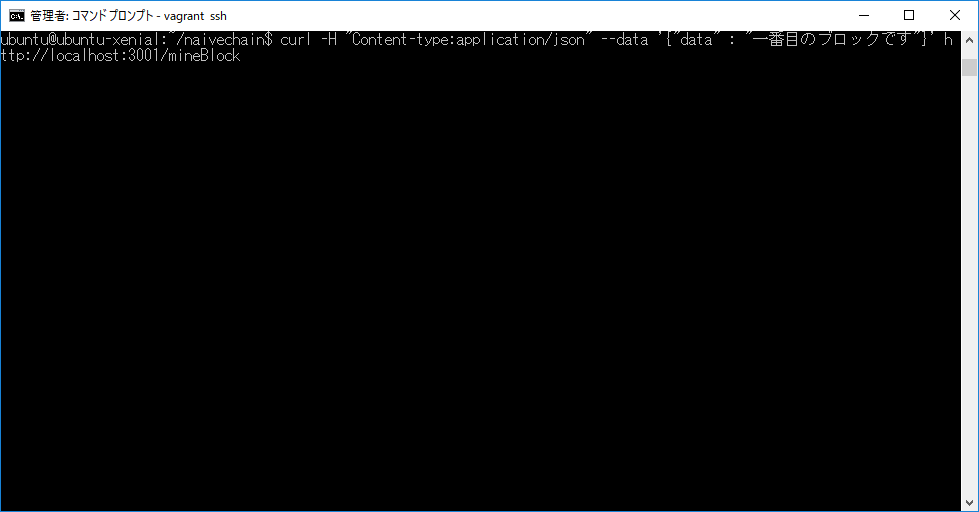
\includegraphics[width=12cm]{no1block.PNG}
\caption{ブロックチェーンへのブロック追加}\label{サンプル図}
\end{figure}

\newpage


\subsection{ブロックの確認}


下記のコマンドを実行した場合,全ブロックチェーンを一覧することができる.

\begin{verbatim}
curl http://localhost:3001/blocks
\end{verbatim}



\begin{figure}[h]
\centering
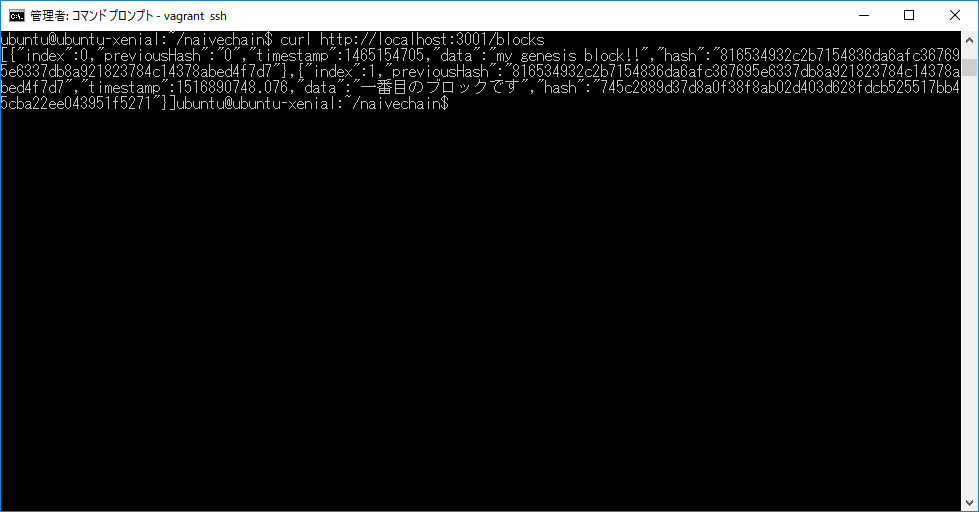
\includegraphics[width=12cm]{no1blockok.PNG}
\caption{ブロックチェーンへのブロック追加}\label{サンプル図}
\end{figure}

先ほど作成,追加したブロックの情報を取得する事ができる.



\newpage

\subsection{他人のノードからのブロックの作成とブロックチェーンへの追加}


以下のコマンドを,同一ネットワーク上で繋がっている仮想マシンンの実装されている他人のノードから入力した場合でもブロックチェーン上にブロックを追加する事ができる.この場合,同一ネットワーク上で繋がっている限り,naivechainのプログラムや,dockerやdocker composeの入っていないノードからでも追加することができる.


以下のように,naivechainの入っているノードipアドレスを含んだurlを記入してブロックに追加する事で,追加するブロックの送り先を指定することができる.


\begin{verbatim}
curl -H "Content-type:application/json" --data
 '{"data" : "鈴木のマシンから二番目のブロック"}'
 http://l0.100.192.78:3001/mineBlock
\end{verbatim}



\begin{figure}[h]
\centering
\includegraphics[width=12cm]{okiadd.PNG}
\caption{同一ネットワーク上でつながっている他人の仮想マシンからのブロックの作成と追加}\label{サンプル図}
\end{figure}


\newpage


\subsection{他人のノードから追加されたブロックの確認}

ブロックの確認で行ったように,下記のコマンドを実行すれば,他ノードから書き込まれたブロックを確認することができる.
\begin{verbatim}
curl http://localhost:3001/blocks
\end{verbatim}

\begin{figure}[h]
\centering
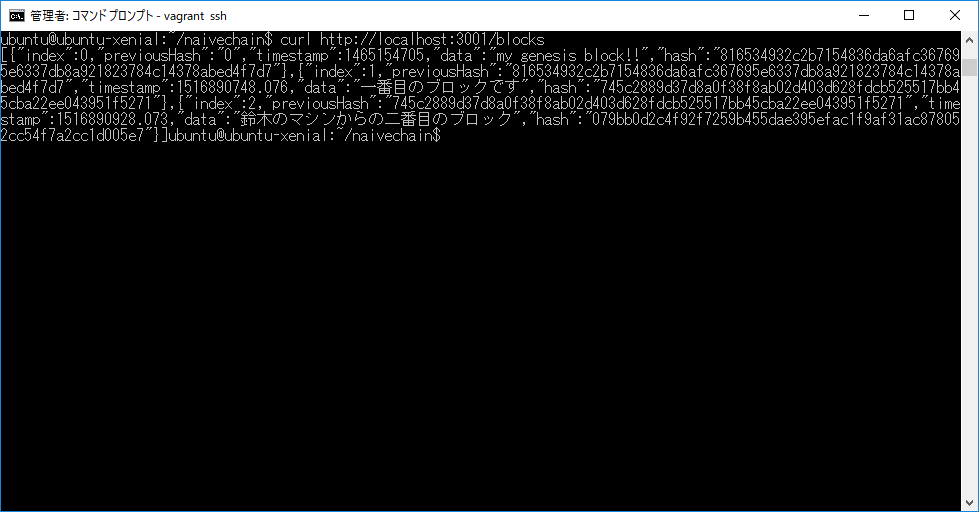
\includegraphics[width=12cm]{no2blockok.PNG}
\caption{同一ネットワーク上でつながっている他人の仮想マシンからのブロックの作成と追加}\label{サンプル図}
\end{figure}


\newpage


\section{Bitcoin Core}
Bitcoin Coreという仮想通貨のアプリケーションでローカルPC上にテストネットワークを構築し,複数のアカウント間でビットコインを送金できた.

\begin{figure}[h]
\centering
\includegraphics[width=12cm]{bitocoin.png}
\caption{Bitcoinの流れ}\label{サンプル図}
\end{figure}
\newpage

\subsection{ブロックの生成}
ビットコインを送金するためにはBTCが必要.ビットコインではブロックを作成する報酬としてBTCを受け取ることができる.ビットコインは報酬を受け取ってから,100ブロック経ないと送金などに利用できないため,最初に101個のブロックを作成した.

\begin{verbatim}
ubuntu@ubuntu-xenial:~/src/bitcoin$ bitcoin-cli -regtest generate 101
[
  "7ef25c199888f2c43295db9546167acf9ff626a84826d10072fa815205ce7d46",
  "7f35aa62a3a56378510b0f3c9fc3a7fa6275cecd73f14ab0b079e057df0b0026",
  "7278455dc0a691391c59895b214cea7aa844199c1436b9ac03a25c834472ddfd",
  "4a3f654bbeeb168dd61faf3b36ee126db166bdab198abf053b6ed24d300cddbd",
  "23a8d44a4e962c6c4beb61b4f26e30bf9ec895d66cd4677743484736128d7877",
  "3fa6a4e518056c4d4c162911623e51e4a8ab8780c0068d7226a0449bc31cba40",
  "646c7a1bd2b66c0ae1914cdf0547b46481597c61b2ddd69b50ac03c807f476b1",
  "307a32619b557d10a8b8b2f2d740b89b8b4b737d77583c5695fe56dd44980ab2",
  "560c454fa7f30142de7c9200164473a82ec09ec27a6e254a418af634b60f6158",
  "585c3a3cc87edb1857008d3c8fef6b75bccaf6b1459f632684d3658d3f100193",
  "1908ca15d23a10ea4a1a51819269a5ef1ba03612c2b960cdba797ff21beb19c9",
  "7d523b9d897531bfe2d0fe3c40e33b1b1655b0c64d588739c7024f6cfc295da9",
  "537725b25b67e5eea1be700f95526a0a4b090573f8498976bcd90bfa055f84de",
  "79d012af4e0ef91f99e737272a106912d5c25940d93fef6e8abe7f25f0d7963f",
  "0c46b586faecbef519a7d709a9a5ca22792929833750f63536abe7b7c0951ed2",
  "346ce292b20fa9e66a40eea731b956144da4c30c34ed1ad486dab692a286962f",
  "15b162514cf2524673875bf09278f62d5ac6b8066bcdd7af8f1bf6dfd610bf56",
  "1510000dae3e601a2dcc464d03be6f5eec7fac4e55ea45e657c3c912db634c25",
  "7988656001fe2d65feebe8cb9759bae3f67f8925c609238008aa292f033f4da8",
  "27f8116b51859ebbfb3eb99d16eb1d9daa3f4f84f2c05b8e24048da2a8f8d9e2",
  "5695233d0603d7b7e3a024f95ccf37b385410e66b3d69fb2a27726299e96e098",
  "575b40c7a6bed5f87689bc278bbffa5450b4a6288b44d9bfb63a66c7ac35e4e3",
  "5c79289002844fef24d560ad1477a0f25b3faea94c9c9db421d615608d44f7f5",
  "3fd93a7637031e6835f9e0458642845f2ba06d862ecbc41da2aa459141140635",
  "4cc549d80c0ba36b063b5eaa4301a74e8fdf871894240347263cb84b96a910b7",
  "63e6fd42ac0c3be1e90e4290f0125cd15d0133ddd40eb77a2b35590f777e1443",
  "612eaeb3b841c1bf6738591207c3831a9f14ee97dc37d3a5dcdbc68a1a4c6c55",
  "2c8abbfead60aa1691461d3dcf3a4e13826891043c9710d62e9ef9a99906fac6",
  "5eb510455813c8815dd02348a7605182df3877e8d84314da671bafd2b2f7c1ed",
  "67f3fe4032165bd02cc143ba409008541e62898af3e0b02e17704b88f0fadefa",
  "1719ada0cc87a4161d0c335f06f5ce754447f650bbb81b56bdad3c875834594c",
  "0ec057a6f1ecbf455acbfe92c18f183a4c3c9c5e52d6524429e39f449971f649",
  "7bb3dc4bc776555258965c4a09cb0227ff51c0cb6f936d3ae2c404df08aba7e4",
  "2ac58ef71bdb7aa24367d03f74a50a3d0bef15b5d36e14d05809702bf870cc61",
  "6b21e97a65fbce0fa3859ad89a9d6d54dca3d0036000c190e205c6a34f0f6d8c",
  "42d902d7cf3d8eead40173c7eb97ae331f414e8ce1e31c3431c6f115eeb30a45",
  "2657af8e06a88e8ccbd4d9db0a01646a49ddbd02876441a75e2d508ba8435f74",
  "7030cae00f73023a9cd28af5a3775c96c064a9151e7d354af8a38c5800b64540",
  "24f49562f97c3fb6ac7959fee4929c9365c97d9b508464d6c19834e06a8782e1",
  "2b056aa1f8839c1fe043c05375164538536dc910b967d10400a1fa3f247e0a36",
  "184652bb56b38dd4687d5c4434d044d967da05412acb0ca1744cd1bdf5bd69eb",
  "4e18a73c050567239fb917a4b62cbdb0a9e98b911485874890bf456c52e4d83d",
  "55d05176368c4f7fed472bcffcda1938d0dae4dd90d285f02562d9073c14ddf1",
  "2d594305f00caa36fdef6167db18689abc5ef3fd94eaff3316e7dab92fb0c472",
  "397648d50807ffebbbb34efb6f1c1301feba6d7d736c88894cc96ce4f951613a",
  "1886fc9bed45adbdd55baf62af14c49ceab460044d2fe9751ddbfb17f59ea884",
  "2268fb65e8a999dd7ca741430614f985bd68e8cae70ae9259107f5142e28d262",
  "234a4961df925d5ffe18b7c6c8121e7ede295a146a0059cab182cd0fe929c285",
  "03b94bf0815b915a98909661d5c6e4a11d37248bede296620dcabb670904b5b2",
  "5c66bd8450743e5da1b5788e1b2ecea6260cd1e9c10e42e41fd19ea4c93d2960",
  "0c49ea0eedb86972290b38137be15f07fc26fcaaed0c173304628759cabdd04c",
  "6be1381e4dc94c3b0a96d46cb9bbd6a20cc0b73e25e3eabbe2ec7931a57133b5",
  "3bb60d0e12a48d98dbbc9d1692aa50972338dc6c95e4dc0515a021f6667e2fe9",
  "2d31ecde9f6771ce638a4afad5fb0b76e0955eadec4af4acb2446b68f9f10a54",
  "46c15a821ec1f78e24e0edc6387c844912d9b13bbe195c052a22fdd0e139f81d",
  "48030cbee97c2824768bbf0c793b6297d6c78007f372ad4fe0a85b08f60f9167",
  "68cda2593cddc4389dc6799d1dad97efc853c66ad28ba59bc77b4b38797246b0",
  "6a1ffab708d366ee2b33b173db82b5f9112251e165829bce9af4ae20f761520d",
  "120da86717ee55eafbfd10439b5fa6a06be8b48d298aafd5d65d48810dfccb53",
  "5f0ee6ff7a84d5bac7af917d7186d21b582ee79641016743a31c2a841144d10e",
  "1f8d24d4e7303928d7a5a8c5992607fa67ffab4c61e0f939ac190eebf1d28194",
  "6b7a8abfb5d46aad2daf842a1d3de0c51683b4a36af349d71dc28b899f01994c",
  "19cc387a183497c034e9156238e8dea2055dd282bab35c4f40088b8be00f563c",
  "678f3aabe7c0587a963cd3deea26ce19b55cf7fa8efb1ad40129b402add5854e",
  "2334ea82c178a4af7fcc4cf34de4d0091995ba927743b3ec6ed04b2543399dde",
  "7ce23f972b108e711d973fdb984cff34748fced371843bccd31e7ac1cfcb577c",
  "1041e3c85623d6b2fcda515a1df8ef6c9280e9c434e446dc1d1005c10944ca99",
  "0a43ad6b6cbae9bbfc1d61dc3b2099fe45229804b4089f3032c5f39ba75427c1",
  "176e12f0adc1ce42d4f3aee818e8e31cad463fe73e87044e598f4c4733aa0568",
  "15d66bf6a71ff8b4596b870416a34073d7160dccd391621350e2bdcc6f82813b",
  "377602127294306c3f0e483e20122cf7a05138e0dd549c2aff682eafdaa2ad6c",
  "1e1e9c8dbc5aeab49d988aa867493558272efcada6585dcd927dac8c3ae416b9",
  "168c5b863835559e97a31ffcbbf16ce5bf8ef0088544bc96b4dc5822c5948ee0",
  "7febdbe9e2c4b2ee878af1cd64553ed1f3307ac82b21c2477a030e2d36503dc8",
  "589c02a454cf81a09d288416c215f811d7523efdf6f3f84962ba702958f72f54",
  "2a7082909cad6c86bcff1d9b0d31014c085f92723ca86349fa48c41eba8a663a",
  "072562cd981196cedd917e8f0a0d3f6a1a535e1a7a487e9b983c1f772e2c2bbb",
  "43d82e8d78ba89d8c44e767f1b7f0b36bfca24cde8e94a1709319d9f8bf55085",
  "51442ccd3796582aefeaccfa1f865df71377f10d9be93778377d919b5cc4bca7",
  "74ae9898c5fa5ae0d812184dc253a0fd0f3499f933a246b877011665f2924ee0",
  "7e8045afc5d4672d09aea83f3231810ba4104f804e35f983ae463dbed3f813a0",
  "2c3769e27e93cf9297eb1cd1c4f7bc46f0714431d053d21a805071565cc5de1b",
  "5a66e5ed427fd5157c811bef29a0edb1c0503c9ec86951a6fc1767841204b478",
  "1927cfc29f42169af7258b7f1c0b3a97aed3fc741928f764329a974e649c656b",
  "2b120249c13ee892e711cfdf7e086f3862c7c0c1d6bf0b9570071f79c68ca950",
  "24fba31ad43d7e35b0c0e0474b88ab9f801a4fec84a8b40c4688f2d810e8f0f3",
  "0c4ab3e8dc4f9b765130bf170b127c291261cac5ddc89ccb0e83fc8a90d3546a",
  "1932cb1a400de7ba40e3d216ca69133dc18deefe447fa564200cfa8631f24077",
  "0045cae03c10d6c7e917f68042976d96096ee0ce0ed2dd807a5c66400053b52d",
  "099c16751261f8584c471cb4cf7f377d8ec2cec57258fd79e94036610390f6af",
  "5caab5807a08380f1d6aabc34572f577ef03ac4298d4468bd34aa1cbe75345d9",
  "4326308d69fedce5bcfec688fbf26b1793614723fec4947f08324e346d75a824",
  "33a700fc422c64ec87fd42c649e3f6fcc9a0fe58605f3fa4dadbfa223c0af943",
  "4122cc92994fe22ab45786334bd025a91e8cdc0123026e0b5a55af6f9fdeb358",
  "007e581ee8406f30f223bd4048b817eb654bfcf376424f4b1d499165e8584359",
  "1b15dc5d48d9b47fe875946607e941fc98de0607b8bd2533a20921c18a8e321a",
  "42fc0d009994d2f98fa2a4206fefde219800d4e4252338cf897f4cc0ac2a98db",
  "4370bb3459050f1e7bc9074c3a2f0718be6d3da0c5231657476696cf08dcf101",
  "32dfeeee098e3db96460e7c5fccbe3b0e38fa5afc7d8464a5d287a14a61ba307",
  "136824554867cf7c86238a3b6d8b9168c7fb7a3454d76e35bb6e955c3bfb05d2",
  "7b05d0f07d737f47166ce21dcfae7646cf4e50d16dfc0b1176af9231e5f17e4a"
]
\end{verbatim}
\newpage

\subsection{ブロック数の確認}
101個のブロックを作成しているので結果は101になる.

\begin{verbatim}
bitcoin-cli -regtest getblockcount

結果:
101
\end{verbatim}


\begin{figure}[h]
\centering
\includegraphics[width=12cm]{caunt.PNG}
\caption{ブロック数の確認}\label{サンプル図}
\end{figure}
\newpage


\subsection{アカウントの生成}
アカウントを生成する.銀行における口座に相当する.この手順によって口座間のBTCのやりとりが可能になる.アカウントは何個でも生成できる.


\begin{verbatim}
bitcoin-clli -regtest getnewaddress testuser2

結果:
mwXKjNW7quodFpoTMnPTwtqCGZ2d9v41KY
\end{verbatim}

\begin{figure}[h]
\centering
\includegraphics[width=12cm]{acaunt.PNG}
\caption{アカウントの生成}\label{サンプル図}
\end{figure}

\newpage


\subsection{残高の確認}
送金処理を行う前に現在の残高を確認する.50BTCが口座に存在している.引数なしでコマンドを実行した場合,マイナーが所有するBTCが表示される.

\begin{verbatim}
bitcoin-clli -regtest getbalance

結果:
50.00000000
\end{verbatim}

\begin{figure}[h]
\centering
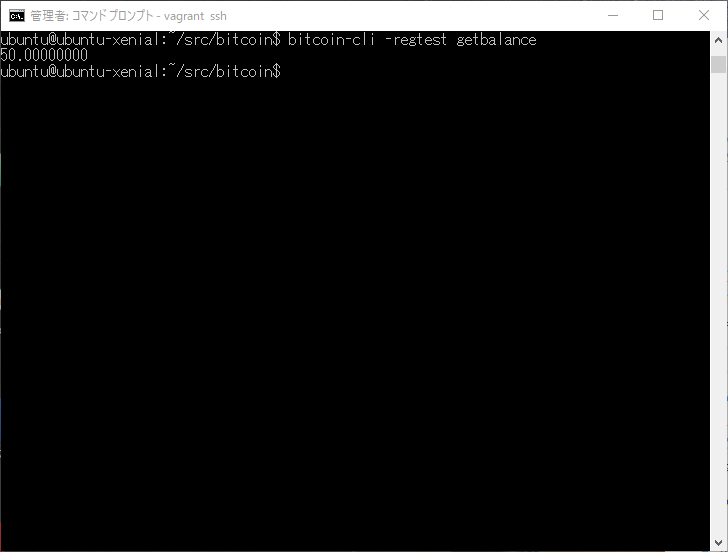
\includegraphics[width=12cm]{zandaka.PNG}
\caption{残高の確認}\label{サンプル図}
\end{figure}



特定アカウントの残高確認.先に作成したアカウントの残高を確認する.testuser2のアカウントにBTCは入っていない.
\begin{verbatim}
bitcoin-clli -regtest getbalance testuser2

結果:
0.00000000
\end{verbatim}

\newpage

\begin{figure}[h]
\centering
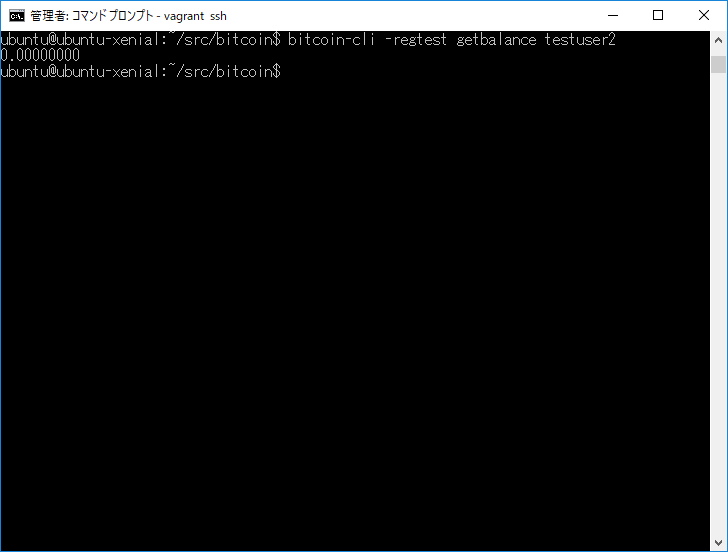
\includegraphics[width=12cm]{zandaka2.PNG}
\caption{特定アカウントの残高確認}\label{サンプル図}
\end{figure}



\newpage



\subsection{送金}
作成したアカウントに実際に送金する.送金処理を行うためには送金先,送金額を指定してトランザクションを発行する必要がある.10BTCをtestuser2に送金した結果を掲載する.結果として表示されたのは,トランザクションを特定するための識別番号(txid).

\begin{verbatim}
bitcoin-cli -regtest sendtoaddress mwXKjNW7quodFpoTMnPTwtqCGZ2d9v41KY 10

結果:
2e45d07dcfb191e0d4f6ca4d1f302600a0e94b02668788ec7fbdcbba0fe723cb
\end{verbatim}

\begin{figure}[h]
\centering
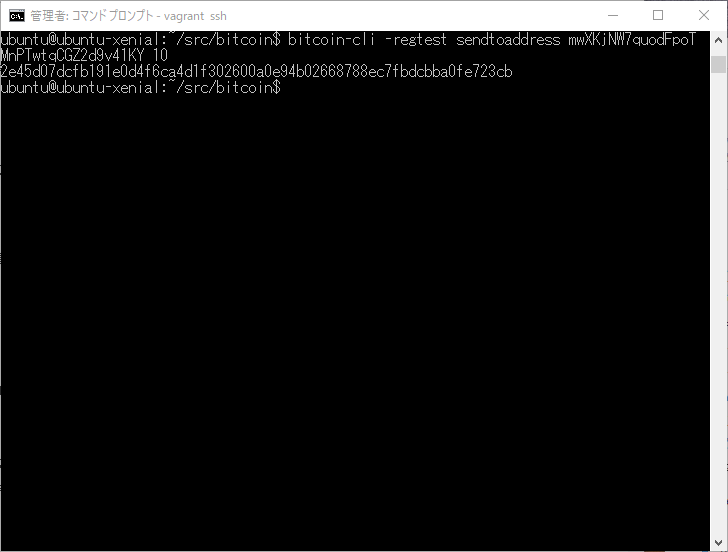
\includegraphics[width=12cm]{sendmoney.PNG}
\caption{送金}\label{サンプル図}
\end{figure}

出力結果は空になる.listunspentは確定したトランザクションを確認するコマンド.
\begin{verbatim}
bitcoin-cli -regtest listunspent

結果:
[
]
\end{verbatim}

\begin{figure}[h]
\centering
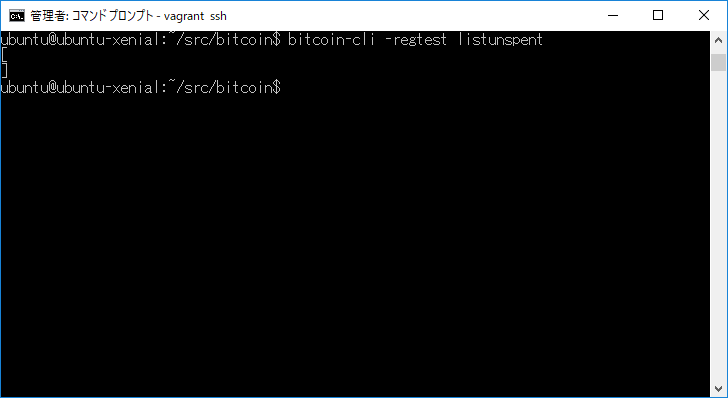
\includegraphics[width=12cm]{tran.PNG}
\caption{トランザクションの確認}\label{サンプル図}
\end{figure}

\newpage


\begin{verbatim}
bitcoin-cli -regtest listunspent 0

結果:
[
  {
    "txid": "2e45d07dcfb191e0d4f6ca4d1f302600a0e94b02668788ec7fbdcbba0fe723cb",
    "vout": 0,
    "address": "mu9gChKwwcmX1uHwRsXM2qKBs9s615T3Pf",
    "scriptPubKey": "76a914958b97b05b8e3d11ce3ec5cde8fef92a05d0fbf188ac",
    "amount": 39.99996160,
    "confirmations": 0,
    "spendable": true,
    "solvable": true,
    "safe": true
  },

\newpage

  {
    "txid": "2e45d07dcfb191e0d4f6ca4d1f302600a0e94b02668788ec7fbdcbba0fe723cb",
    "vout": 1,
    "address": "mwXKjNW7quodFpoTMnPTwtqCGZ2d9v41KY",
    "account": "testuser2",
    "scriptPubKey": "76a914af93e82677e868782ae9a260f2eea64a2014783688ac",
    "amount": 10.00000000,
    "confirmations": 0,
    "spendable": true,
    "solvable": true,
    "safe": true
  }
]
\end{verbatim}

先ほど表示されたトランザクションの識別番号と同じ値で,14行目の"address"に送金先アカウント,17行目に送金額が出力される.また5行目の"address"が送金元アカウントであり,7行目の"amount"に送金後の送金元アカウントの金額が表示されている.

\newpage

\subsection{マイニング}
未確定のトランザクションを確定するためにマイニングを実行した.ブロックチェーンではマイニングによってトランザクションがブロックに書き込まれることで送金が確定する.

\begin{verbatim}
bitcoin-cli -regtest generate 1

結果:
[
  "16d9d752607d47d67a944a6bb7d04178e598407c07b187e34b6238868261a970"
]
\end{verbatim}

\subsection{送金の確認}
\begin{verbatim}
bitcoin-cli -regtest getbalance testuser2

結果:
10.00000000
\end{verbatim}

アカウントに送金額の10BTCが存在していることがわかる.送金に成功した.


\newpage

\chapter{考察}

データの改ざんが困難なブロックチェーン上で誰もが記録を閲覧できる本研究は,Akatsukiのようなソーシャルゲームサービスを提供している会社の意図的な不正と,ユーザー側の一方的な誤解を防ぐ証明として役立つのではないかと考えられる.しかしユーザーが意図的に誤った情報をブロックチェーンに書き込んでしまう可能性もあるので,ブロックチェーンにブロックを追加する際には有料アイテムの抽選結果をユーザーによって改変できない仕組みが必要である.


\newpage

\chapter{結論}

以上の結果から,ブロックチェーンに記録されたゲーム内乱数の信憑性は高いと言える.今後は抽選結果をコンピュータが自動的に判断してブロックチェーンに追加するシステムを実装することが今後の課題である.


\bibliographystyle{junsrt}
\bibliography{biblio}%「biblio.bib」というファイルが必要.



\chapter*{謝辞}\addcontentsline{toc}{chapter}{謝辞}

本研究を進めるにあたり,ご指導を頂いた卒業論文指導教員の矢吹太朗准教授に感謝致します.先生には研究以外にも多くのことを教えていただきました.研究の進め方や論文の書き方など,ひとかたならぬご指導をいただきました.言葉を尽くしても足りないほど感謝しております.本当にありがとうございました.また、研究や日常の議論を通じて多くの発見をさせてくれた矢吹研究室の皆様,その他本研究や大学生活全体を通してかかわっていただいた皆様にも多大なる感謝の意をここに表します.



\end{document}
